\documentclass{uspBeamer}

%============================================================
%-------------------------- SETUP ---------------------------
%============================================================

\author[Silva, J. T.]{Jonathan Tobias da Silva}
\title[Análise de vulnerabilidades em redes OPC UA industriais]{Análise de vulnerabilidades em redes OPC UA industriais}
\subtitle{Qualificação para mestrado em Engenharia Elétrica}
\institute[USP]{EESC/SEL/USP}
\date{\today}
\def \advisor{Prof. Dr. Ivan Nunes da Silva}
% \def \supervisor{Prof. Dr. André Luis Dias}
\subject{USP Presentation}
\graphicspath{ {Public/Images/} }

%============================================================
%----------------------- LOCAL CONFIG -----------------------
%============================================================

\titlegraphic{
	\begin{tikzpicture}[remember picture, overlay]
		\node[xshift=-14cm, yshift=-8cm] at (current page.center){ % right=0.2cm - good as well
			
\includegraphics[width=60pt]{logo_eesc_horizontal-transparente.png}
		};
	\end{tikzpicture}
}
\usebackgroundtemplate{
	
\includegraphics[width=\paperwidth,height=\paperheight]{bodyEESC2.png}
}

%--------- CRONOGRAMA ---------
\newcommand*{\thead}[1]{\multicolumn{1}{|c|}{\bfseries #1}}
\newcommand{\x}[1]{\cellcolor{mainColor1} #1}
\newcommand{\y}[1]{\cellcolor{mainColor2} #1}
%\def\arraystretch{1}
\setlength\tabcolsep{2pt}

%============================================================
%------------------------- DOCUMENT -------------------------
%============================================================

\begin{document}
	
    %________________________________________________________
	%-------------------- INIT PAGE -------------------------

    {
		\usebackgroundtemplate{
\includegraphics[width=\paperwidth,height=\paperheight]{titleEESC.png}}
		\begin{frame}[plain]
		\end{frame}
	}

	%________________________________________________________
	%-------------------- TITLE PAGE ------------------------
	
	{
		\usebackgroundtemplate{
\includegraphics[width=\paperwidth,height=\paperheight]{backgroundEESC.png}}
		\begin{frame}[plain]
			\maketitle
		\end{frame}
	}
	
	%________________________________________________________
	%------------------- TOC - PART  ------------------------

	% \part{Demonstrativa de elementos}
	\begin{frame}{Agenda}
		\tableofcontents
	\end{frame}

    \section{Introdução}

    \begin{frame}{Resumo}
        \begin{figure}
            \begin{columns}
                \begin{column}{.5\textwidth}
                    \begin{wideitemize}
                        \item Crescimento avançado da transformação digital
                        \item Sistemas de Automação e Controle Industriais
                        \item Protocolo OPC UA
                        \item Preocupação com a segurança cibernética
                    \end{wideitemize}
                \end{column}
                \begin{column}{.5\textwidth}
                    \begin{figure}
                        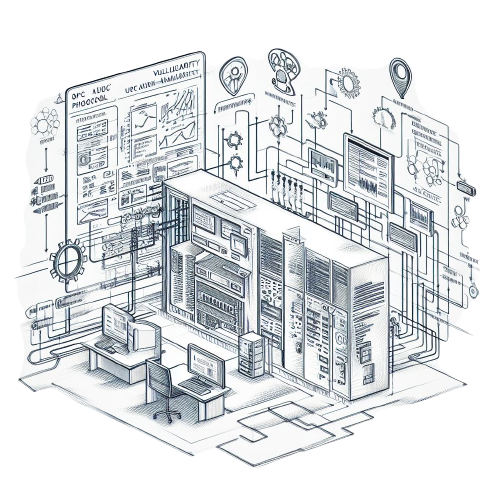
\includegraphics[width=0.8\textwidth]{master.png}
                    \end{figure}
                \end{column}
            \end{columns}
        \end{figure}
    \end{frame}

    \begin{frame}{Proposta inicial vs atual}
        \begin{figure}
            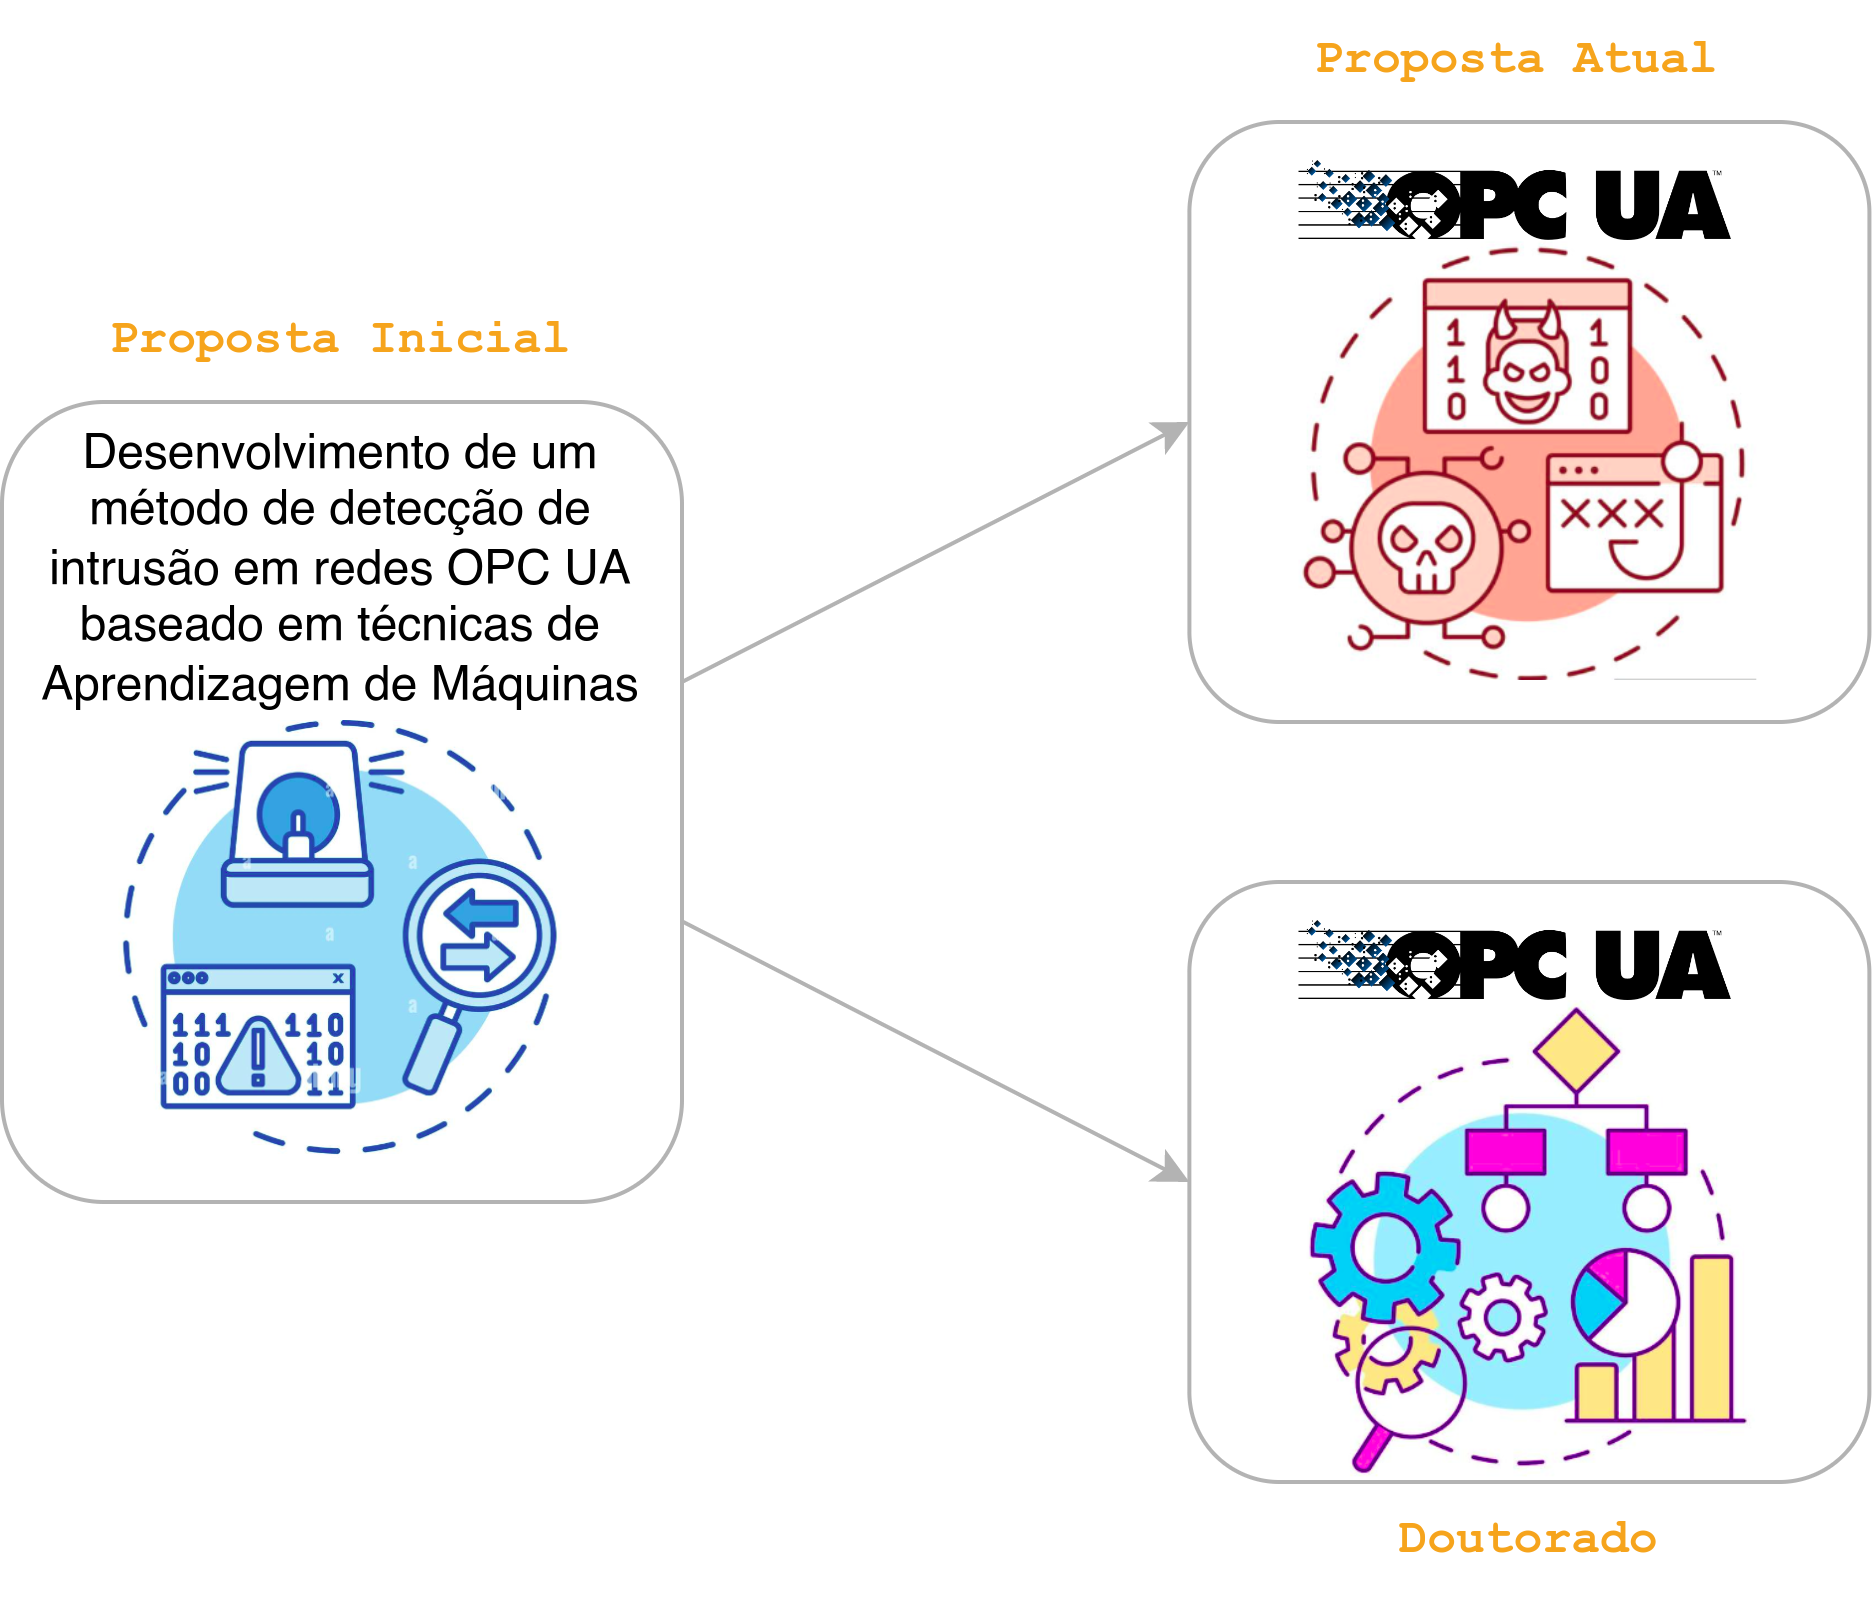
\includegraphics[scale=0.63]{proposta.png}
        \end{figure}
    \end{frame}

    \subsection{Motivação e Justificativa}

    \begin{frame}{Motivação}
        \begin{columns}
            \begin{column}{.5\textwidth}
                \begin{wideitemize}
                    \uncover<1->{\item Aumento nos casos de ataques cibernéticos em CPPSs}
                    \uncover<2>{
                    \item \textit{Industrial Internet of Things}
                    \item Sistemas de Controle e Automação Industrial
                    \item \textit{Service Orientated Architecture} (SOA)
                    \item \textit{Open Process Automation Standards} (O-PAS)
                    \begin{itemize}
                        \item Baseado na IEC 62443
                        \item Possuí uma parte específica para Security
                        \item Comunicação baseada no OPC UA
                    \end{itemize}
                    \item \textit{Cybersecurity}
                    \item Convergência IT/OT
                    }
                \end{wideitemize}
            \end{column}
            \begin{column}{.5\textwidth}
                \only<1>{
                    \begin{block}{Maroochy Shire - 2000}
                        O sistema de controle da estação de tratamento de água, inundando o terreno do hotel com esgoto bruto
                    \end{block}
                    \begin{block}{U.S. Federal Aviation Administration - 2009}
                        \textit{Hackers} invadiram várias vezes os sistemas de apoio à missão de controle de tráfego aéreo
                    \end{block}
                    \begin{block}{Iran's nuclear system - 2011}
                        \textit{Hackers} interromperam o sistema nuclear do Irã utilizando o worm \textbf{Stuxnet}
                    \end{block}
                    \begin{block}{Ukrainian power grid - 2016}
                        30 subestações de energia foram derrubadas por seis horas, afetando cerca de 80.000 pessoas
                    \end{block}
                }
                \only<2>{
                    \begin{figure}
                        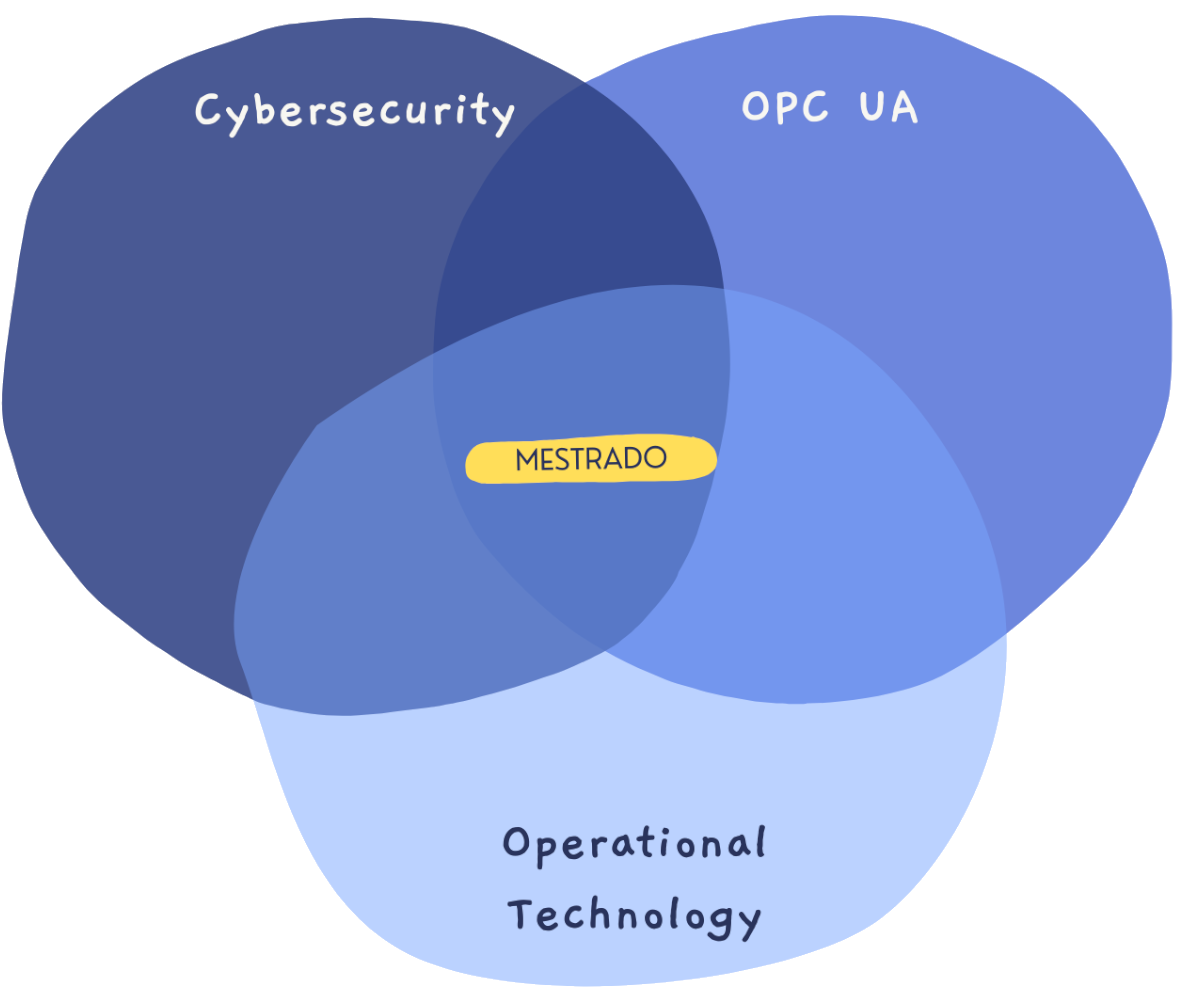
\includegraphics[scale=0.6]{pillars.png}
                    \end{figure}
                }
            \end{column}
        \end{columns}
    \end{frame}

    \begin{frame}{Pesquisa bibliográfica}{OPC UA}
        \begin{columns}
            \begin{column}{0.4\textwidth}
                \begin{wideitemize}
                    \item Base de dados
                    \begin{wideitemize}
                        \item IEEEXplore
                    \end{wideitemize}
                    \item Termos de pesquisa
                    \begin{wideitemize}
                        \item \code{OPC UA} ou
                        \item \code{OPC Unified Architecture} ou
                        \item \code{OPC:UA} ou
                        \item \code{OPC-UA}
                    \end{wideitemize}
                \end{wideitemize}
            \end{column}
            \begin{column}{0.6\textwidth}
                \begin{wideitemize}
                    \item Filtros de pesquisa
                    \begin{wideitemize}
                        \item \textbf{Idioma:} Inglês
                        \item \textbf{Data:} 2018 - 2023
                        \item \textbf{Critérios de exclusão:}
                        \begin{itemize}
                            \item OPC UA aplicado na indústria ou IoT não é o foco principal da publicação;
                            \item O OPC UA é referenciado na publicação, mas não é um tópico relevante da mesma;
                            \item Publicações que se concentram em \textit{marketing} de produtos e não priorizam o OPC UA como protocolo central ou recurso.
                        \end{itemize}
                    \end{wideitemize}
                    \item Publicação: \textbf{IEEE/IAS International Conference on Industry Applications}
                    \begin{wideitemize}
                        \item \textit{A survey on OPC UA protocol: overview, challenges and opportunities}
                    \end{wideitemize}
                \end{wideitemize}
            \end{column}
        \end{columns}
    \end{frame}

    \begin{frame}{Pesquisa bibliográfica}{OPC UA + Analise de Vulnerabilidades}
        \begin{columns}
            \begin{column}{0.4\textwidth}
                \begin{wideitemize}
                    \item Bases de dados
                    \begin{wideitemize}
                        \item IEEEXplore
                        \item Scopus
                        \item Web Of Science
                    \end{wideitemize}
                    \item Termos de pesquisa
                    \begin{wideitemize}
                        \item \code{OPC UA} (ou derivados) e
                        \item \code{Vulnerabilities} ou
                        \item \code{Vulnerabilities Analysis} ou
                        \item \code{Vulnerabilities Assessment}
                    \end{wideitemize}
                \end{wideitemize}
            \end{column}
            \begin{column}{0.6\textwidth}
                \begin{wideitemize}
                    \item Filtros de pesquisa
                    \begin{wideitemize}
                        \item \textbf{Idioma:} Inglês
                        \item \textbf{Data:} 2013 - 2023
                    \end{wideitemize}
                    \item Principais referências
                    \begin{wideitemize}
                        \item Simulating and Detecting Attacks of Untrusted Clients in OPC UA Networks \cite{neu2019}
                        \item Vulnerabilities of the Open Platform Communication Unified Architecture Protocol in Industrial Internet of Things Operation \cite{shin2022}
                        \item Security Analysis of OPC UA in Automation Systems for IIoT \cite{varadarajan2022}
                    \end{wideitemize}
                \end{wideitemize}
            \end{column}
        \end{columns}
    \end{frame}
    
    \subsection{Objetivos}

    \begin{frame}
        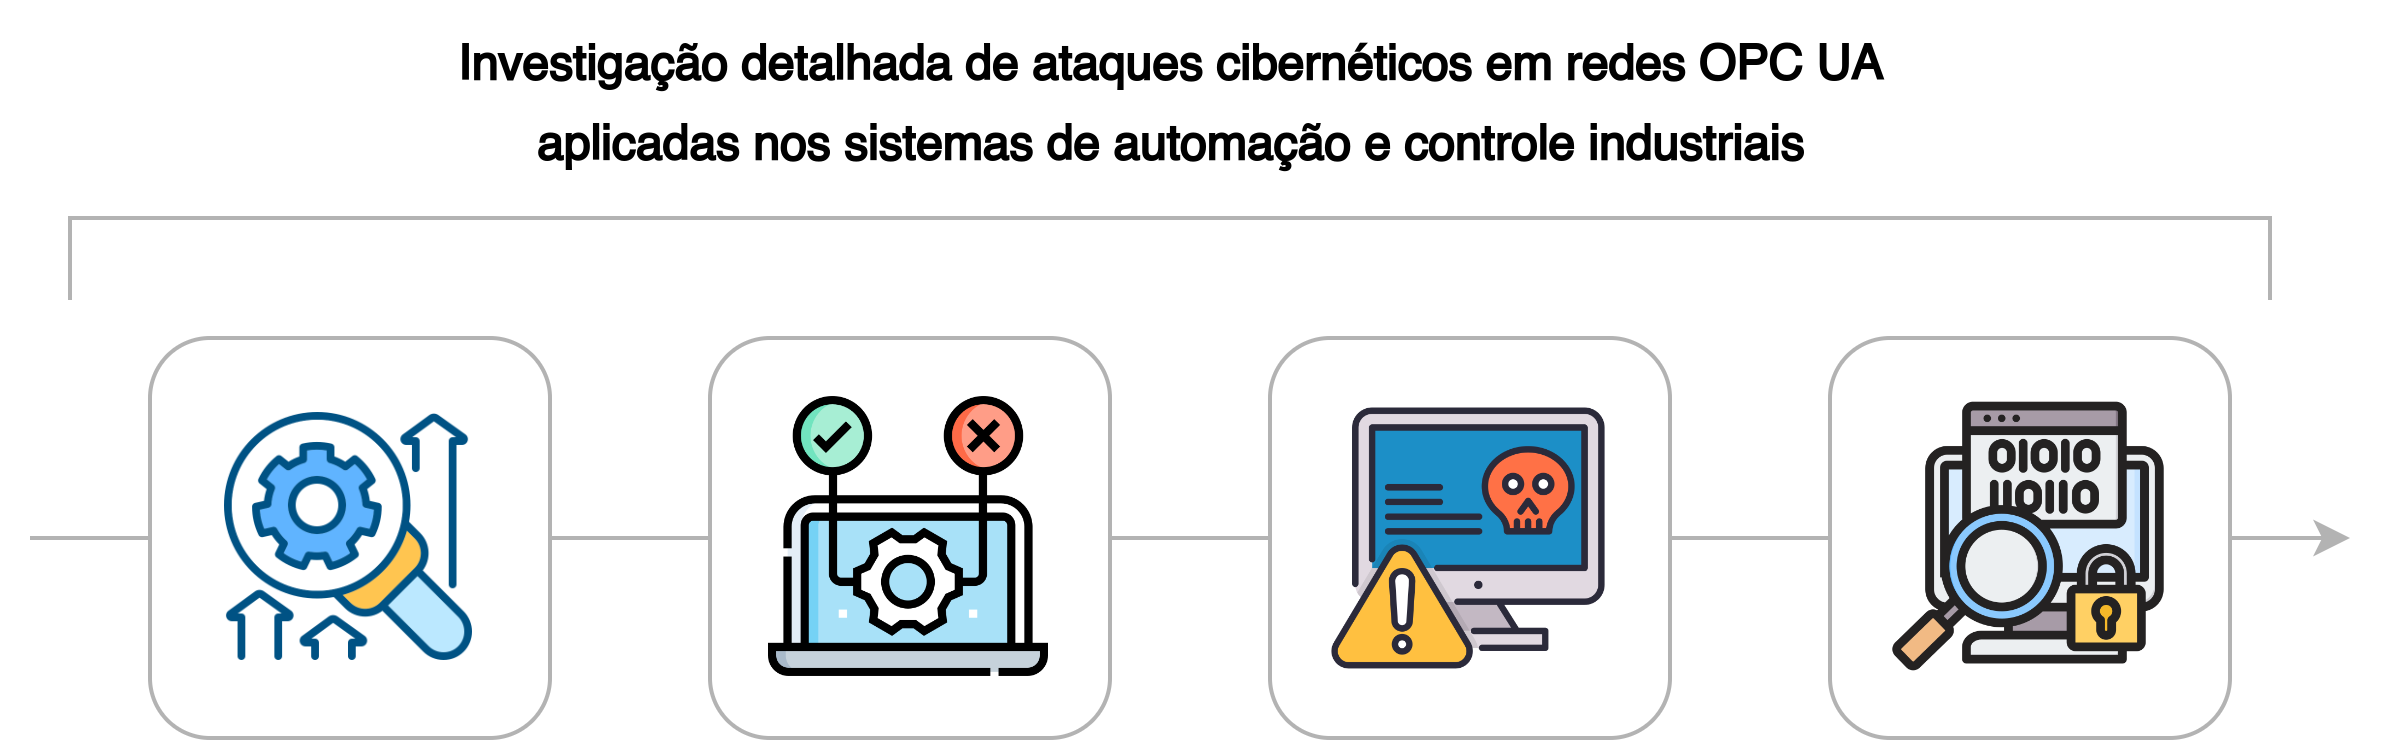
\includegraphics[scale=0.9]{objetivos.png}
    \end{frame}

    \section{Referencial Teórico}
    \subsection{Protocolos IoT e IIoT}

    \begin{frame}{Principais aspectos do OPC UA}
        \begin{columns}
            \begin{column}{.5\textwidth}
                \begin{wideitemize}
                    \item Padrão de comunicação industrial interoperável
                    \item Segurança integrada
                    \item Plataforma agnóstica
                    \item Modelo de informação unificado
                    \item Arquitetura Orientada a Serviços (SOA)
                    \item Robusto e confiável
                    \item Suporte a dados complexos em tempo real
                    \item Serviços Web
                \end{wideitemize}
            \end{column}
            \begin{column}{.5\textwidth}
                \begin{figure}
                    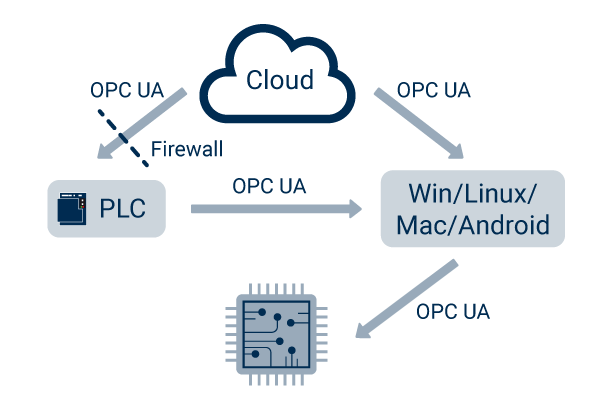
\includegraphics[scale=0.30]{opcua1.png}
                \end{figure}
                \footnotetext{\href{https://www.opc-router.com/what-is-opc-ua/}{OPC Router - What is OPC UA?}}
            \end{column}
        \end{columns}
    \end{frame}

    \begin{frame}{OPC UA}{\textit{Address Space} e \textit{Information Model}}
        \begin{figure}
            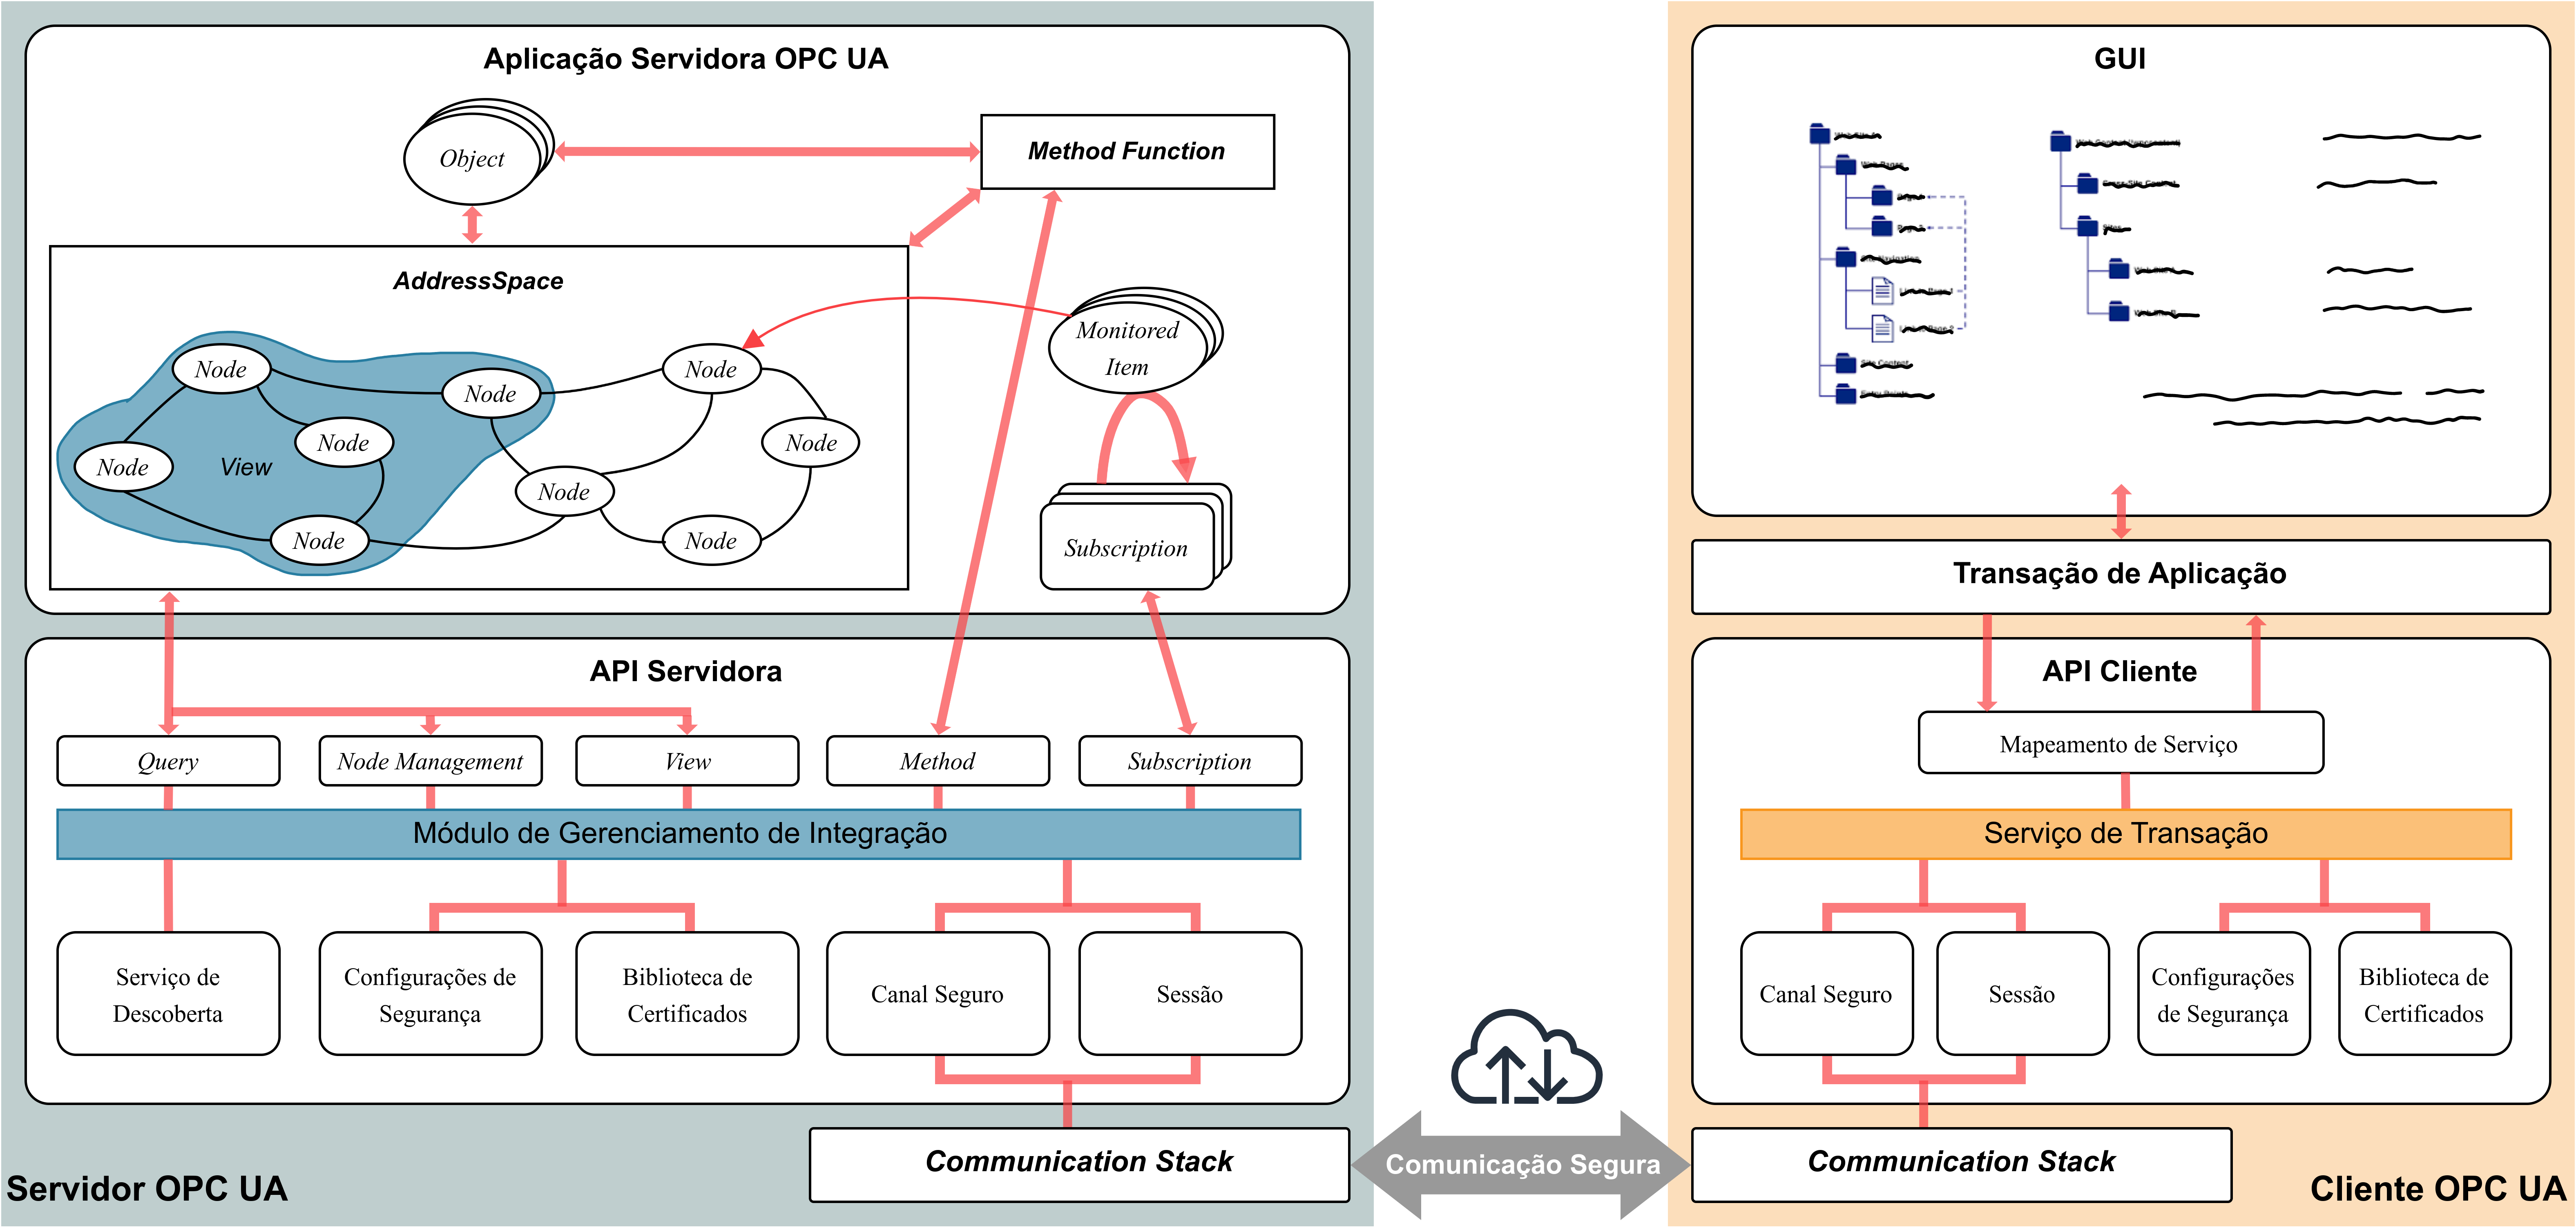
\includegraphics[width=.9\textwidth]{opcuaClientServerArc1.png}
        \end{figure}
    \end{frame}

    \begin{frame}{OPC UA}{Escopo de proteção}
        \begin{columns}
            \begin{column}{.3\textwidth}
                \begin{wideitemize}
                    \item Tríade CIA:
                    \begin{wideitemize}
                        \item Confidencialidade
                        \item Integridade
                        \item Disponibilidade
                    \end{wideitemize}
                    \item \textit{Framework} AAA:
                    \begin{wideitemize}
                        \item Autenticação
                        \item Autorização
                        \item Auditoria
                    \end{wideitemize}
                \end{wideitemize}
            \end{column}
            \begin{column}{.7\textwidth}
                \begin{figure}
                    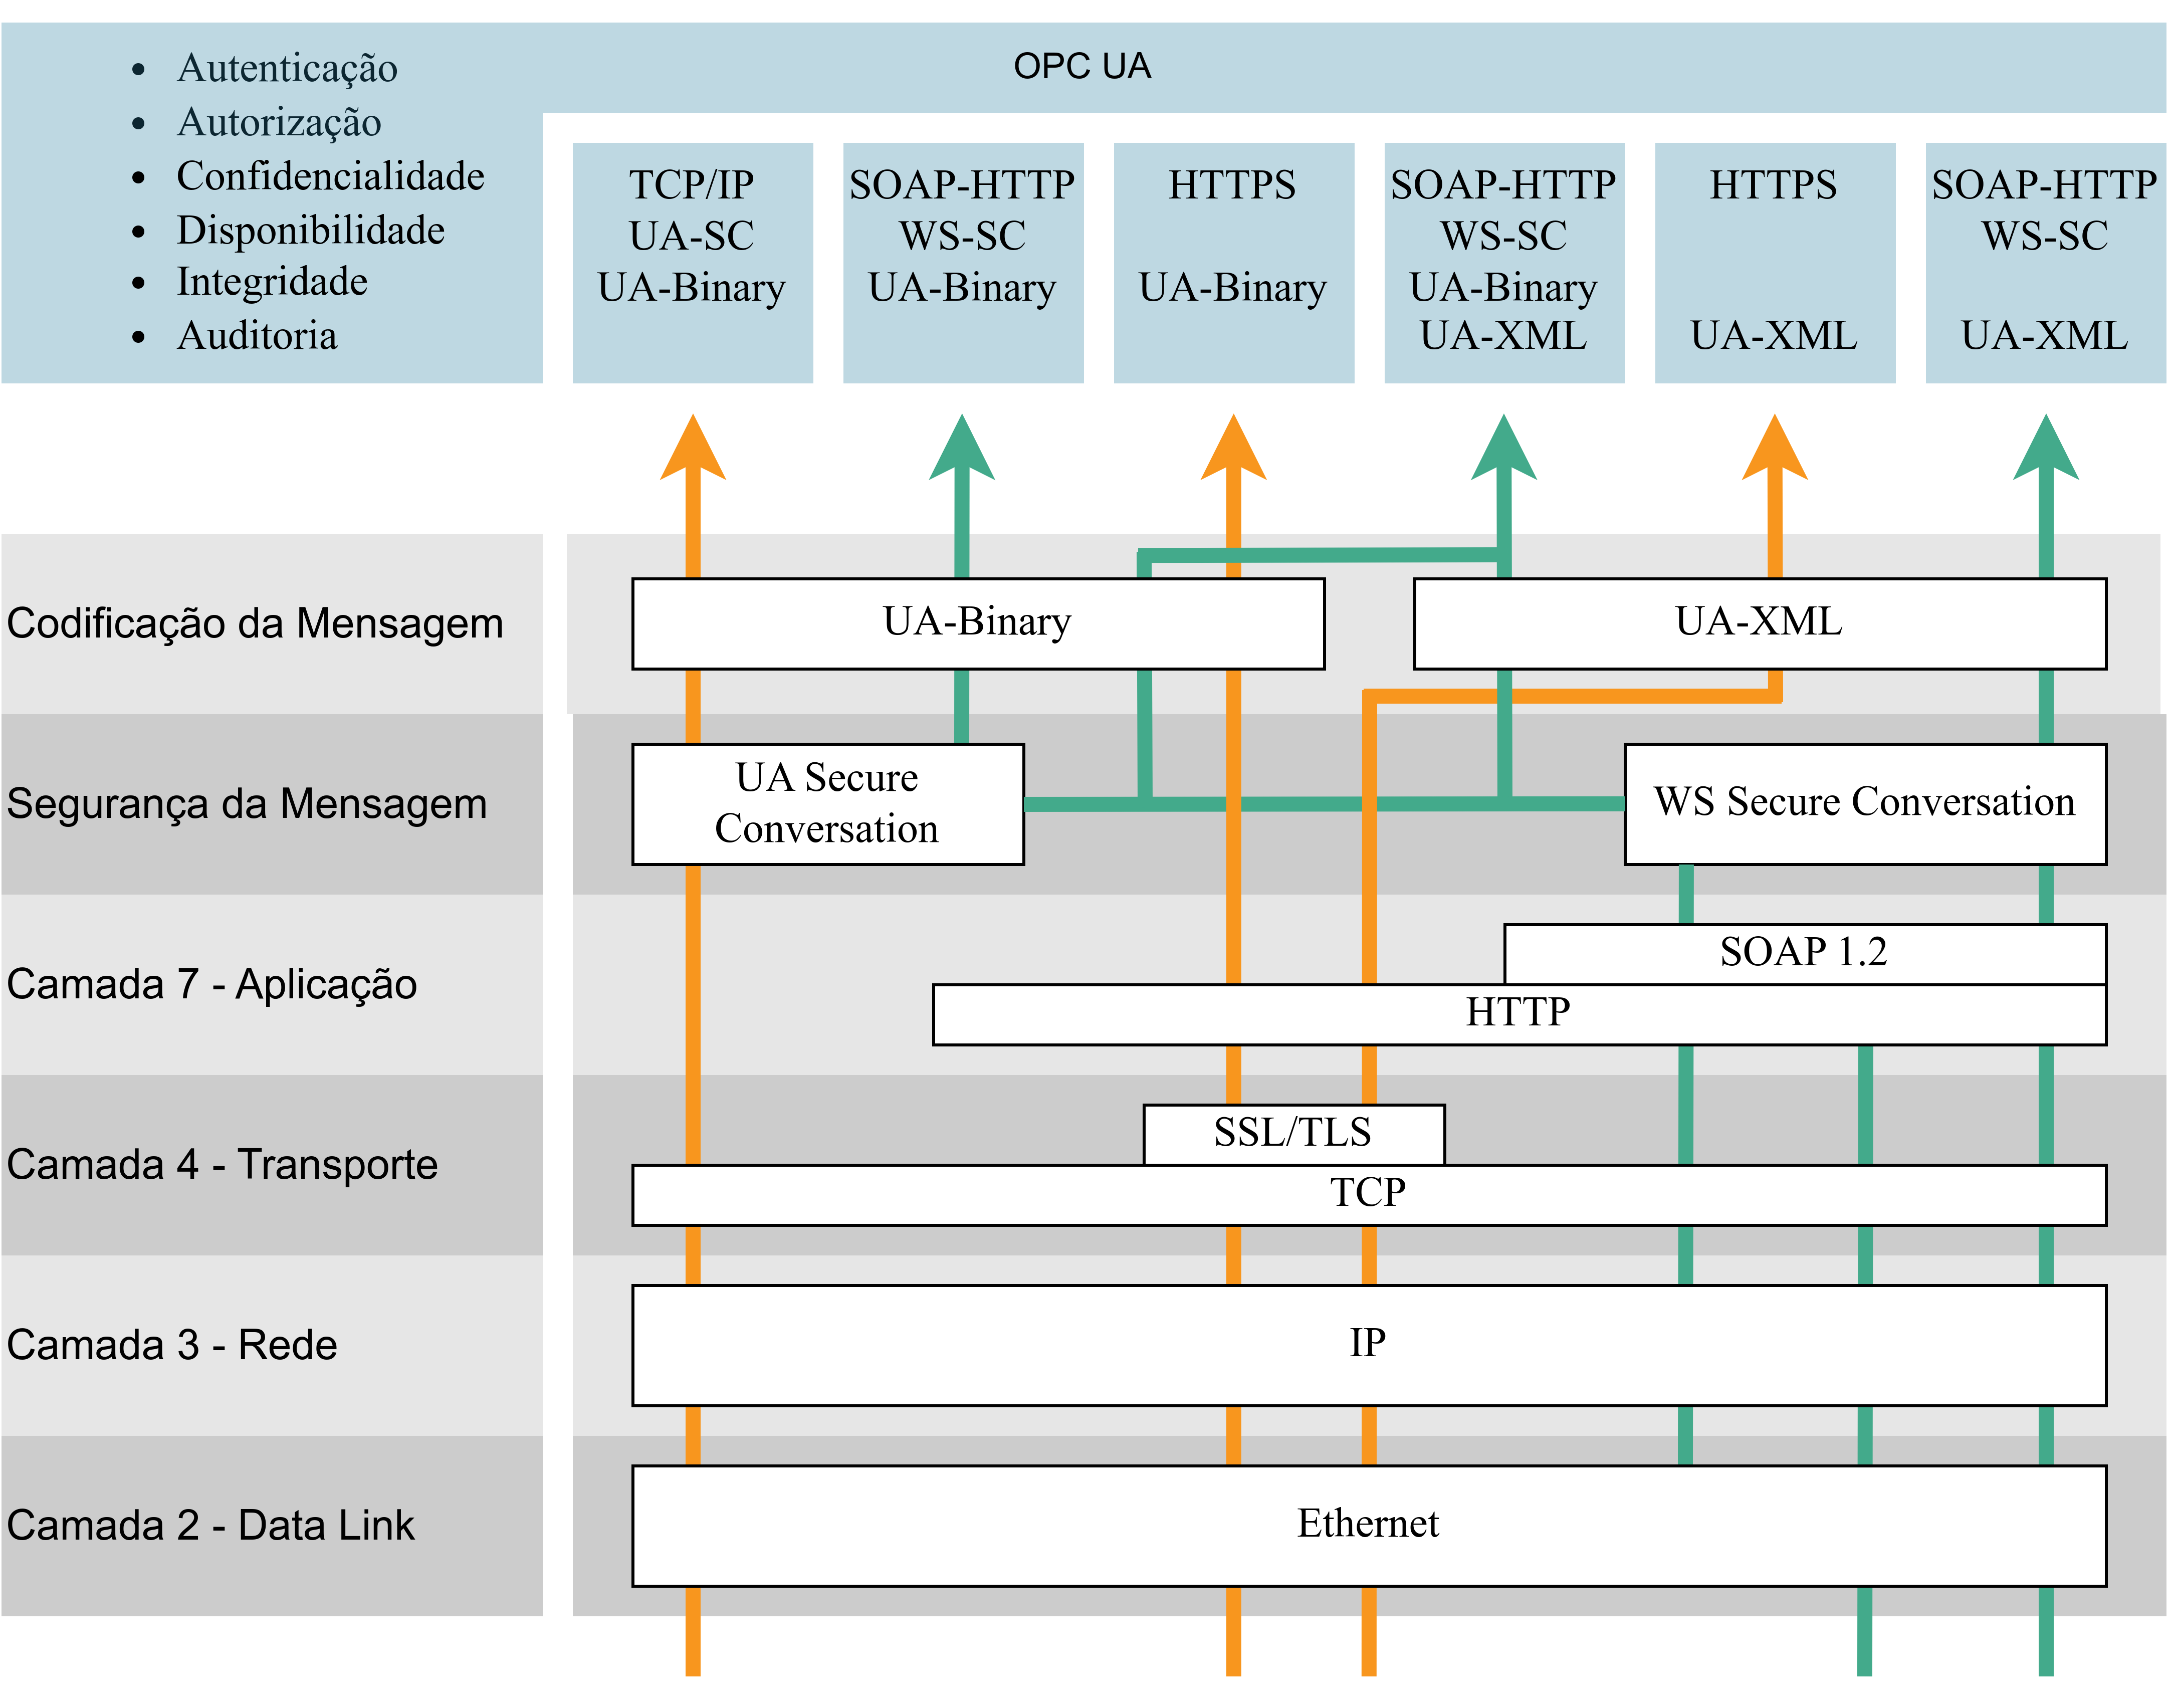
\includegraphics[height=.83\textheight]{ua-osi.png}
                \end{figure}
            \end{column}
        \end{columns}
    \end{frame}

    \begin{frame}{OPC UA}{Processo de conexão segura}
        \begin{figure}
            \only<1>{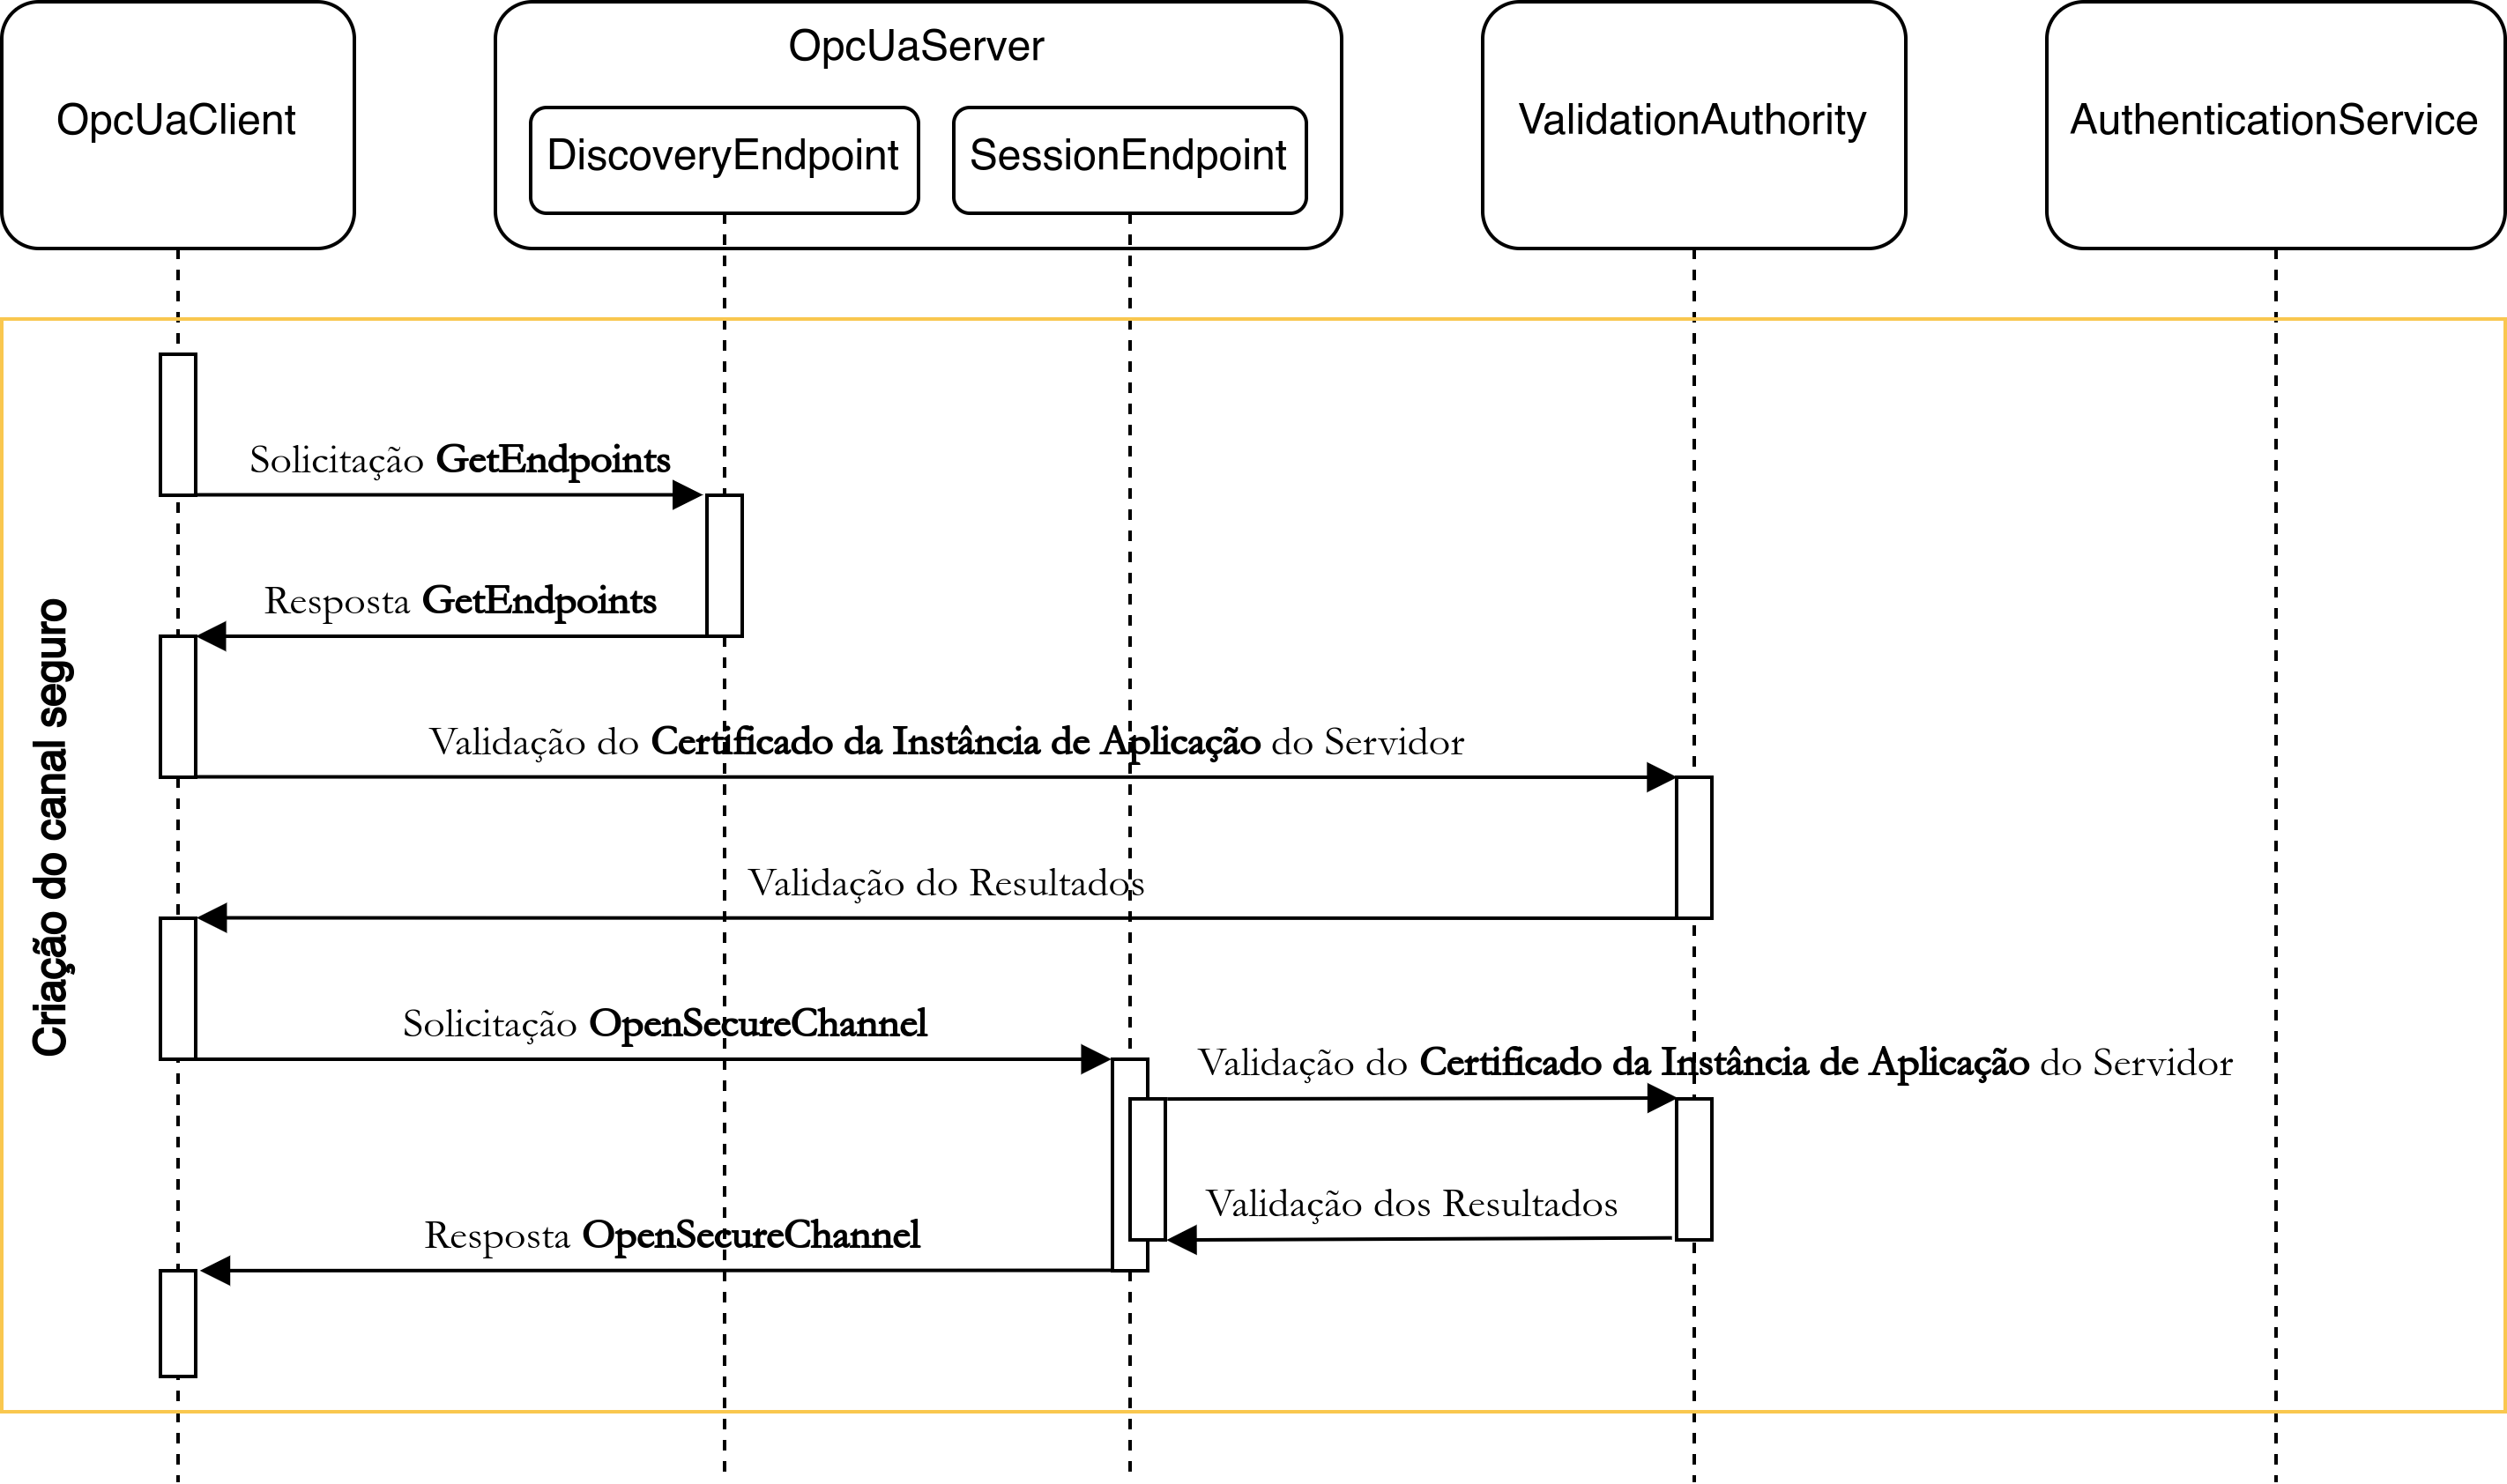
\includegraphics[width=.7\textwidth]{seqConn-1.png}}
            \only<2>{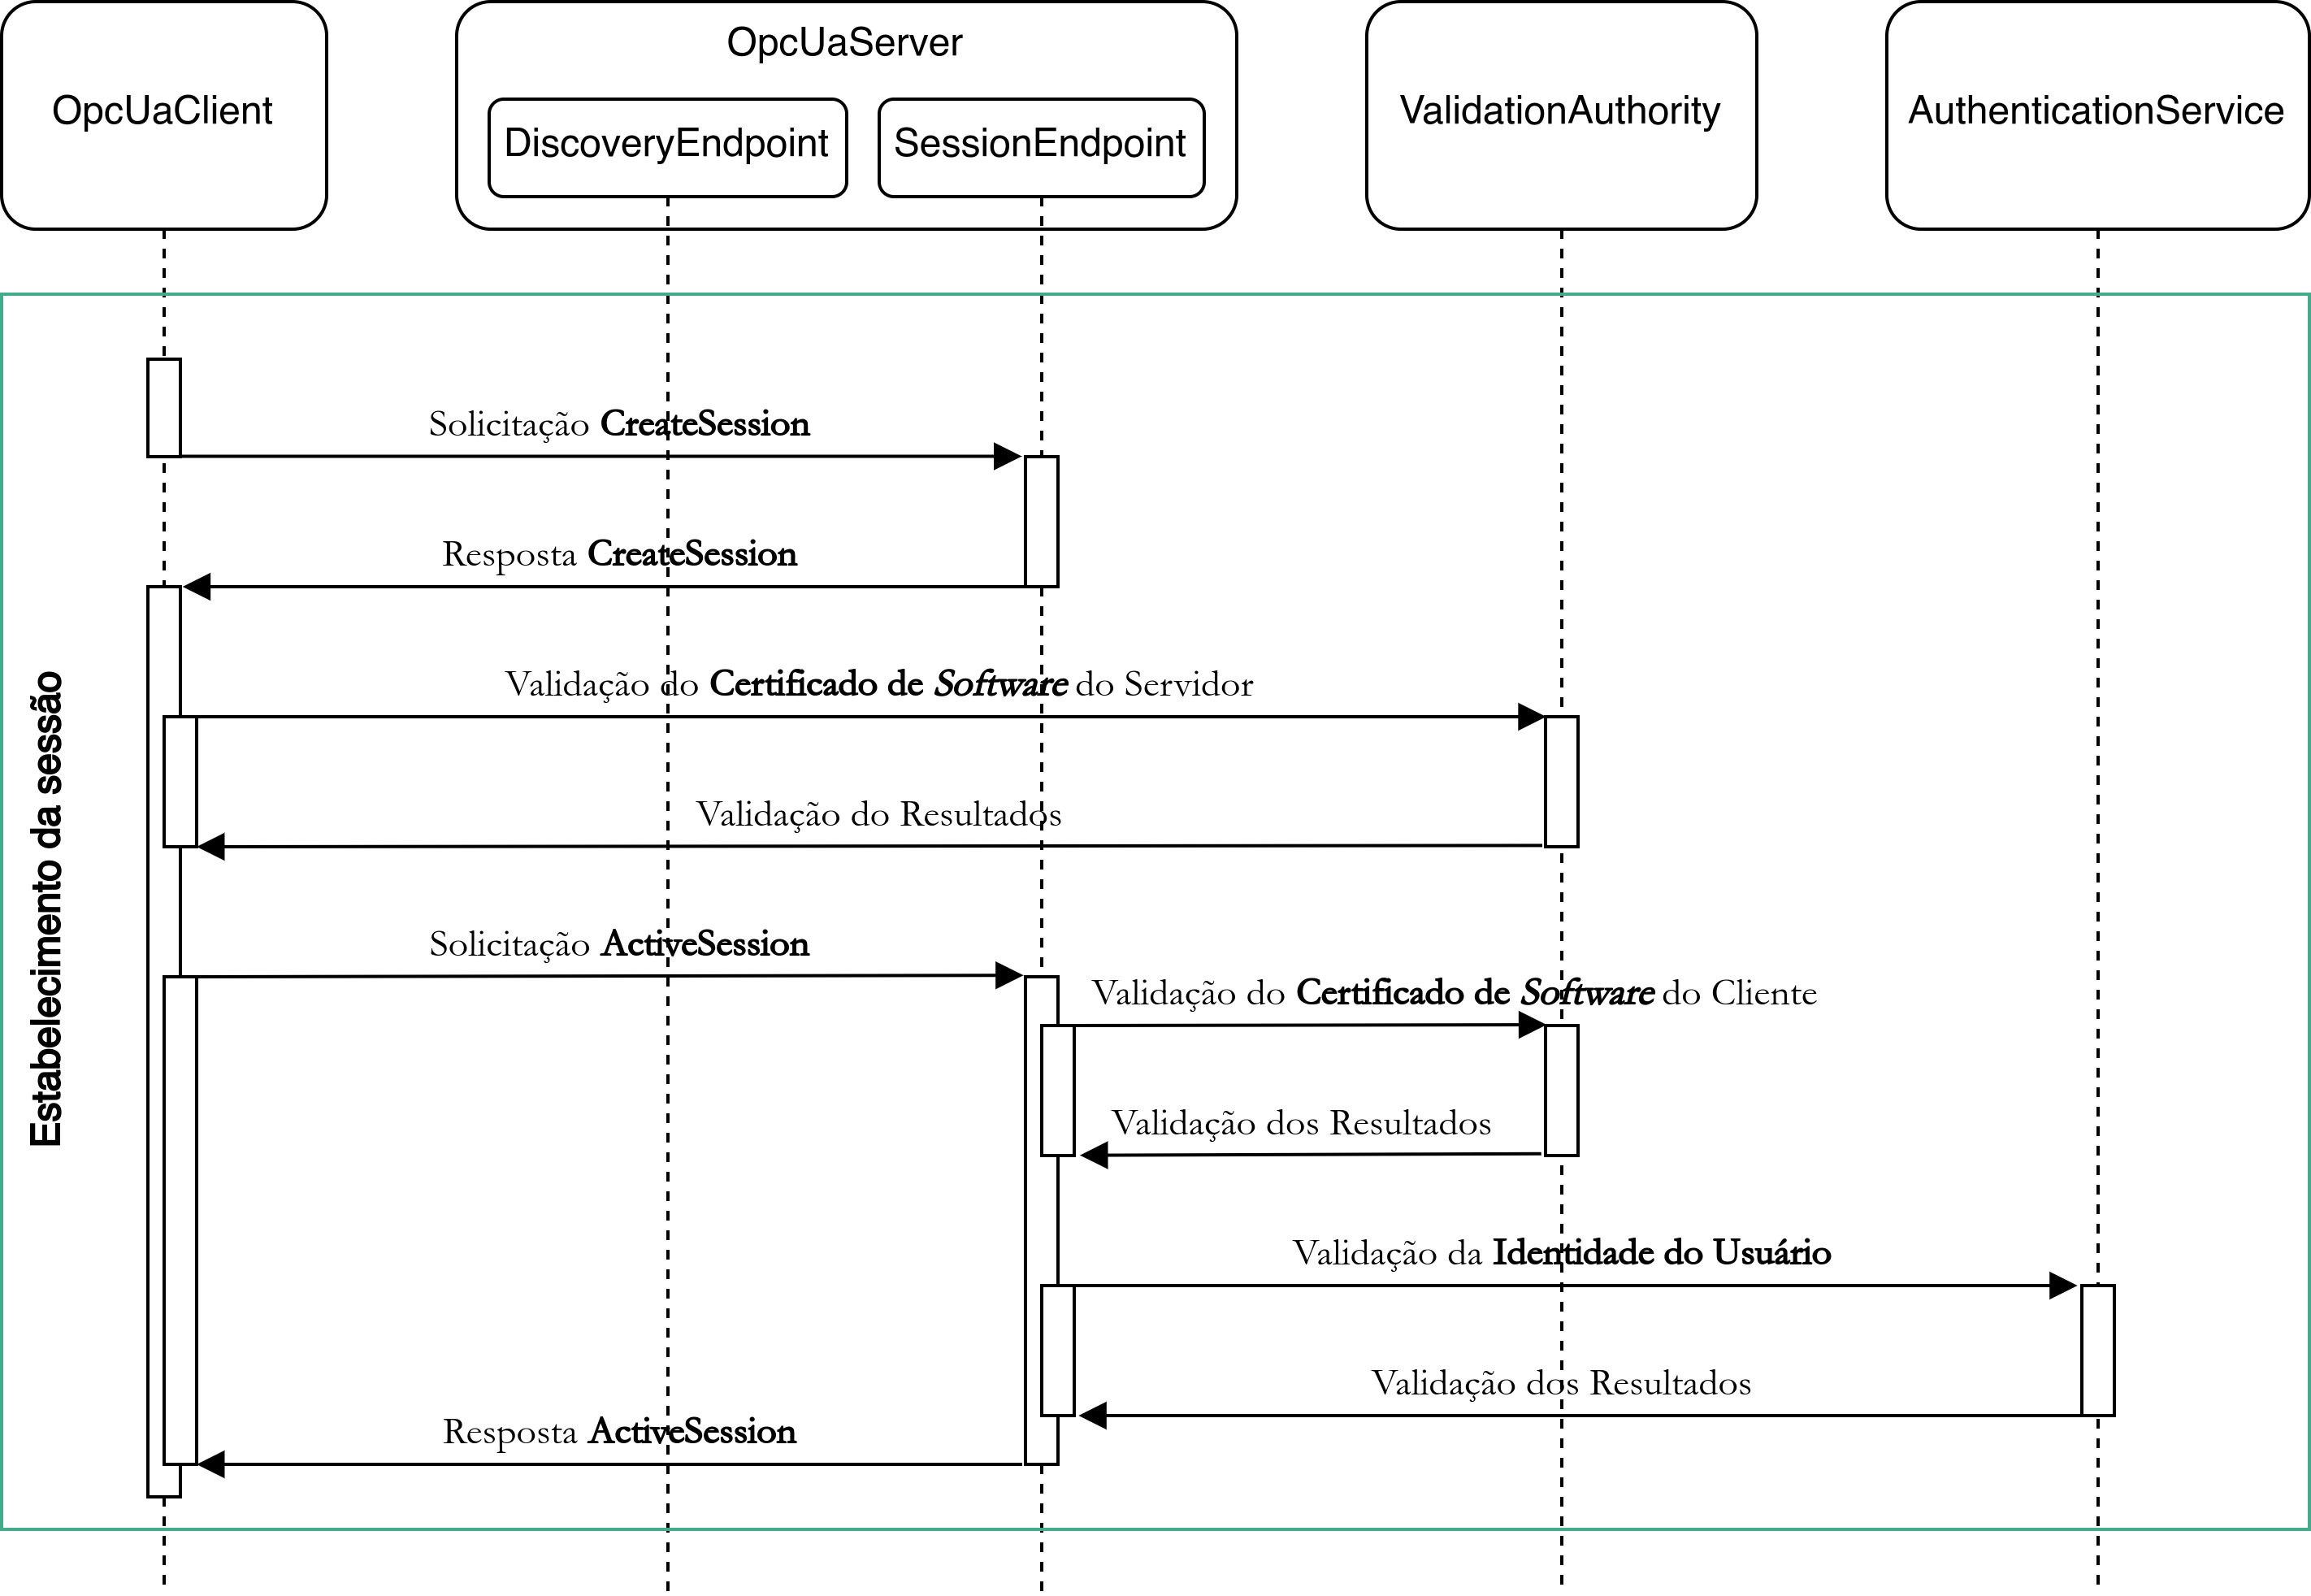
\includegraphics[width=.7\textwidth]{seqConn-2.png}}
            \only<3>{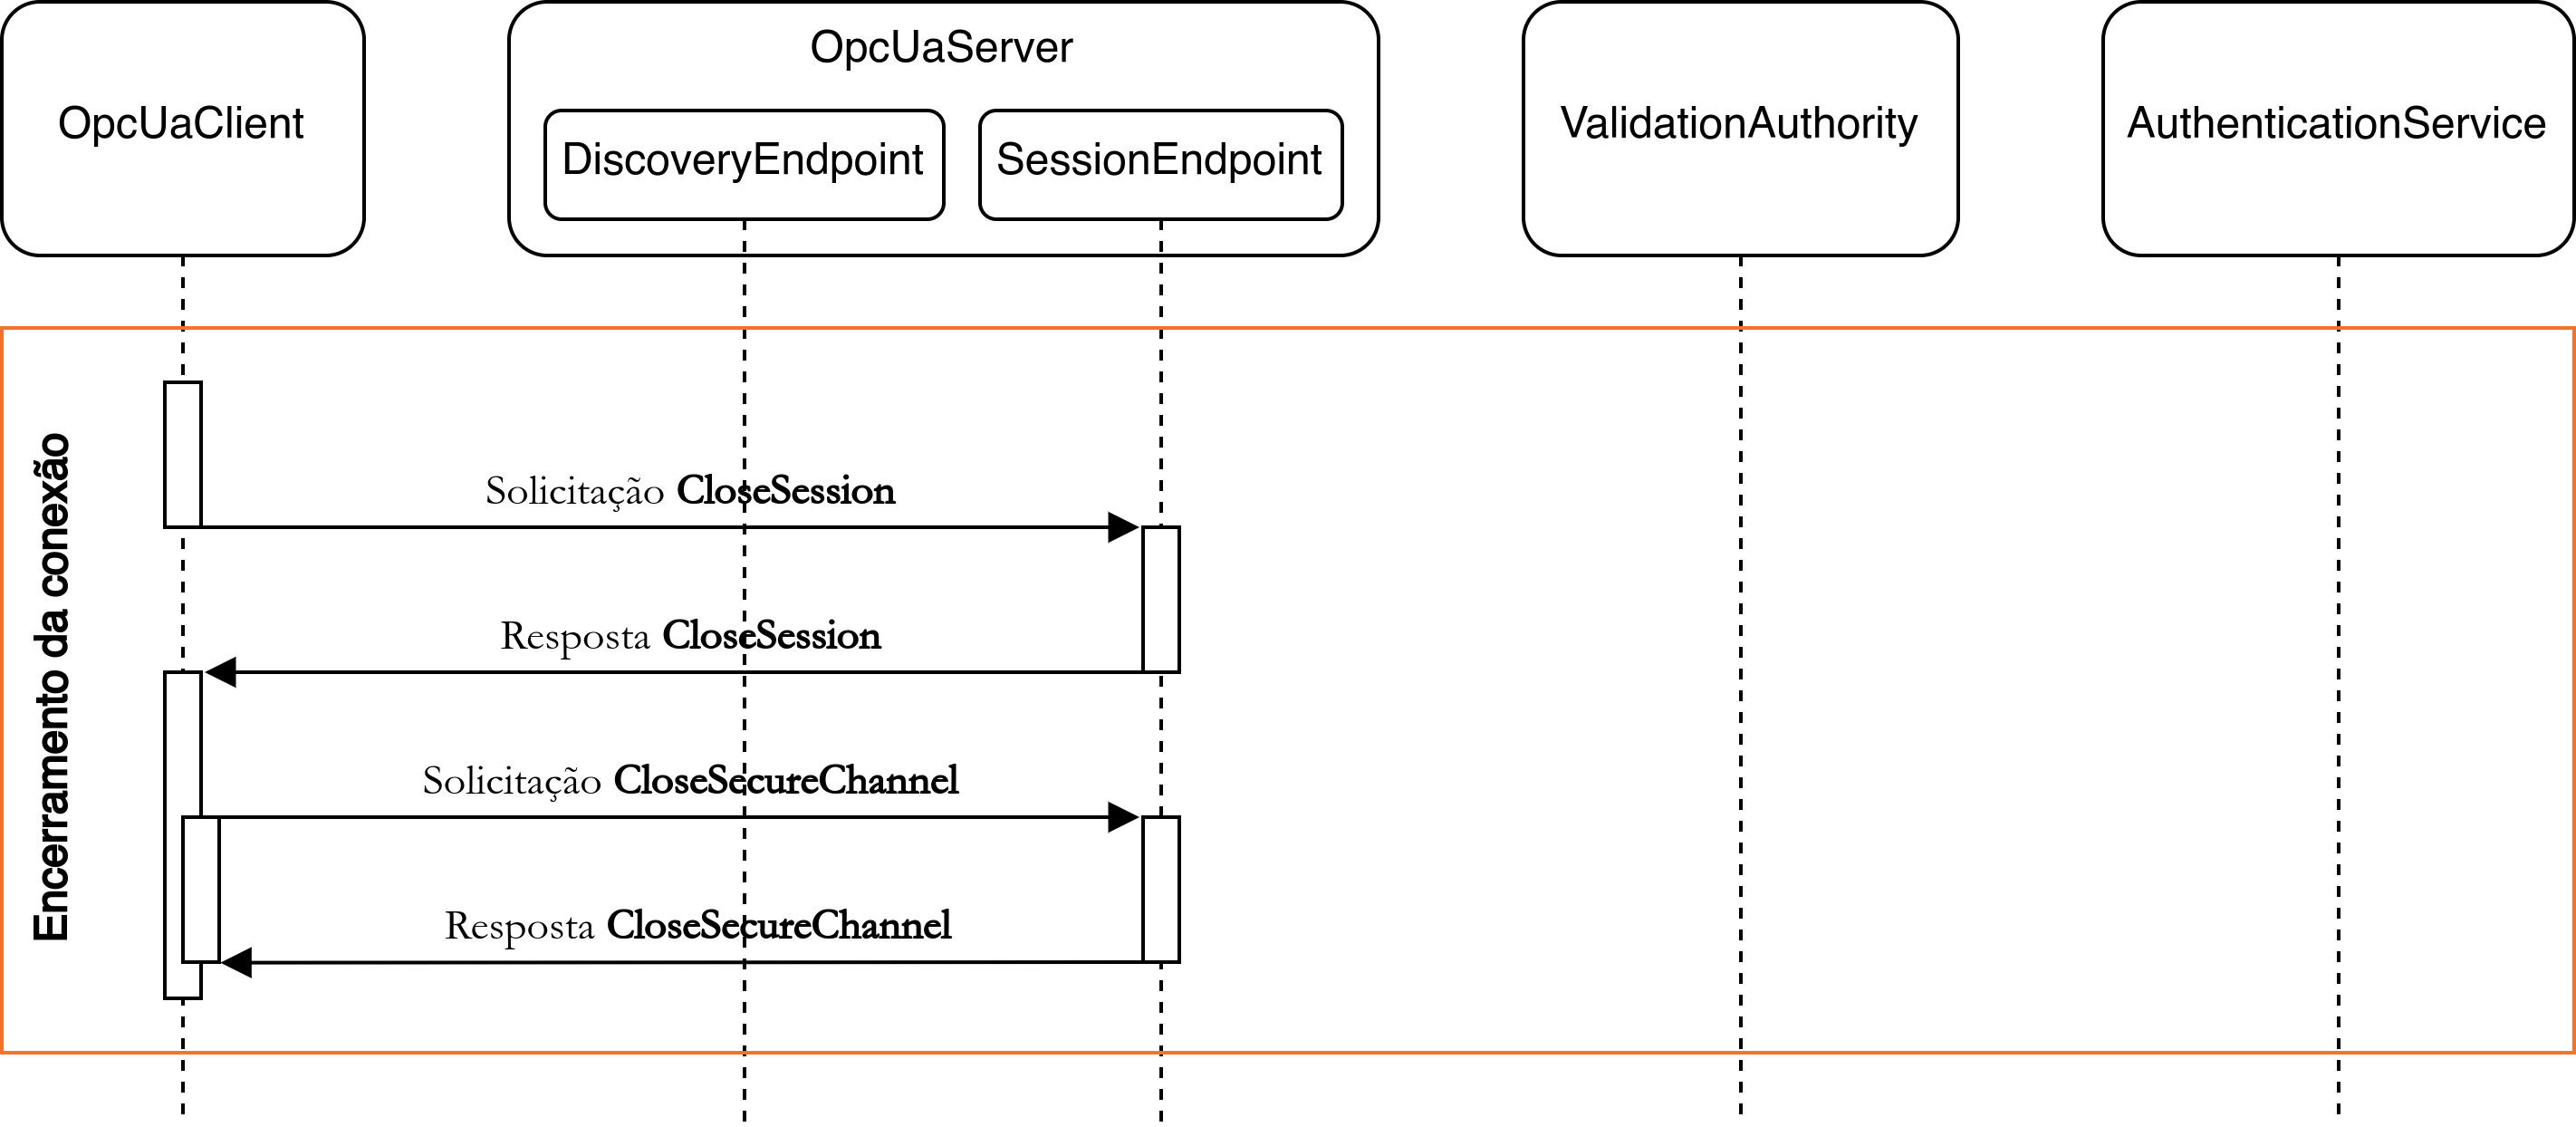
\includegraphics[width=.7\textwidth]{seqConn-3.png}}
        \end{figure}
    \end{frame}

    \subsection{\textit{Cybersecurity}}

    \begin{frame}{Convergência IT/OT}
        \begin{figure}
            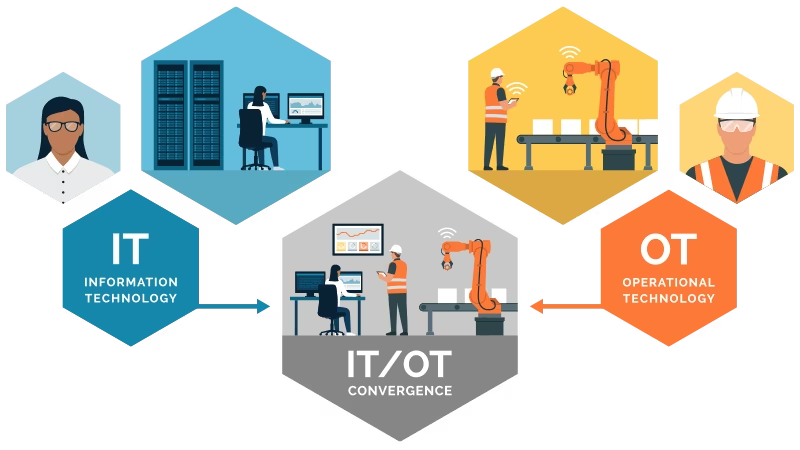
\includegraphics[width=.8\textwidth]{convergenceitot.png}
        \end{figure}
        \footnotetext{\href{https://www.connection.com/brand/cisco/manufacturing-iot/cisco-iot-manufacturing-solutions}{Connection - Cisco IoT Manufacturing Solutions}}
    \end{frame}

    \begin{frame}{Ataques cibernéticos}
        \begin{figure}
            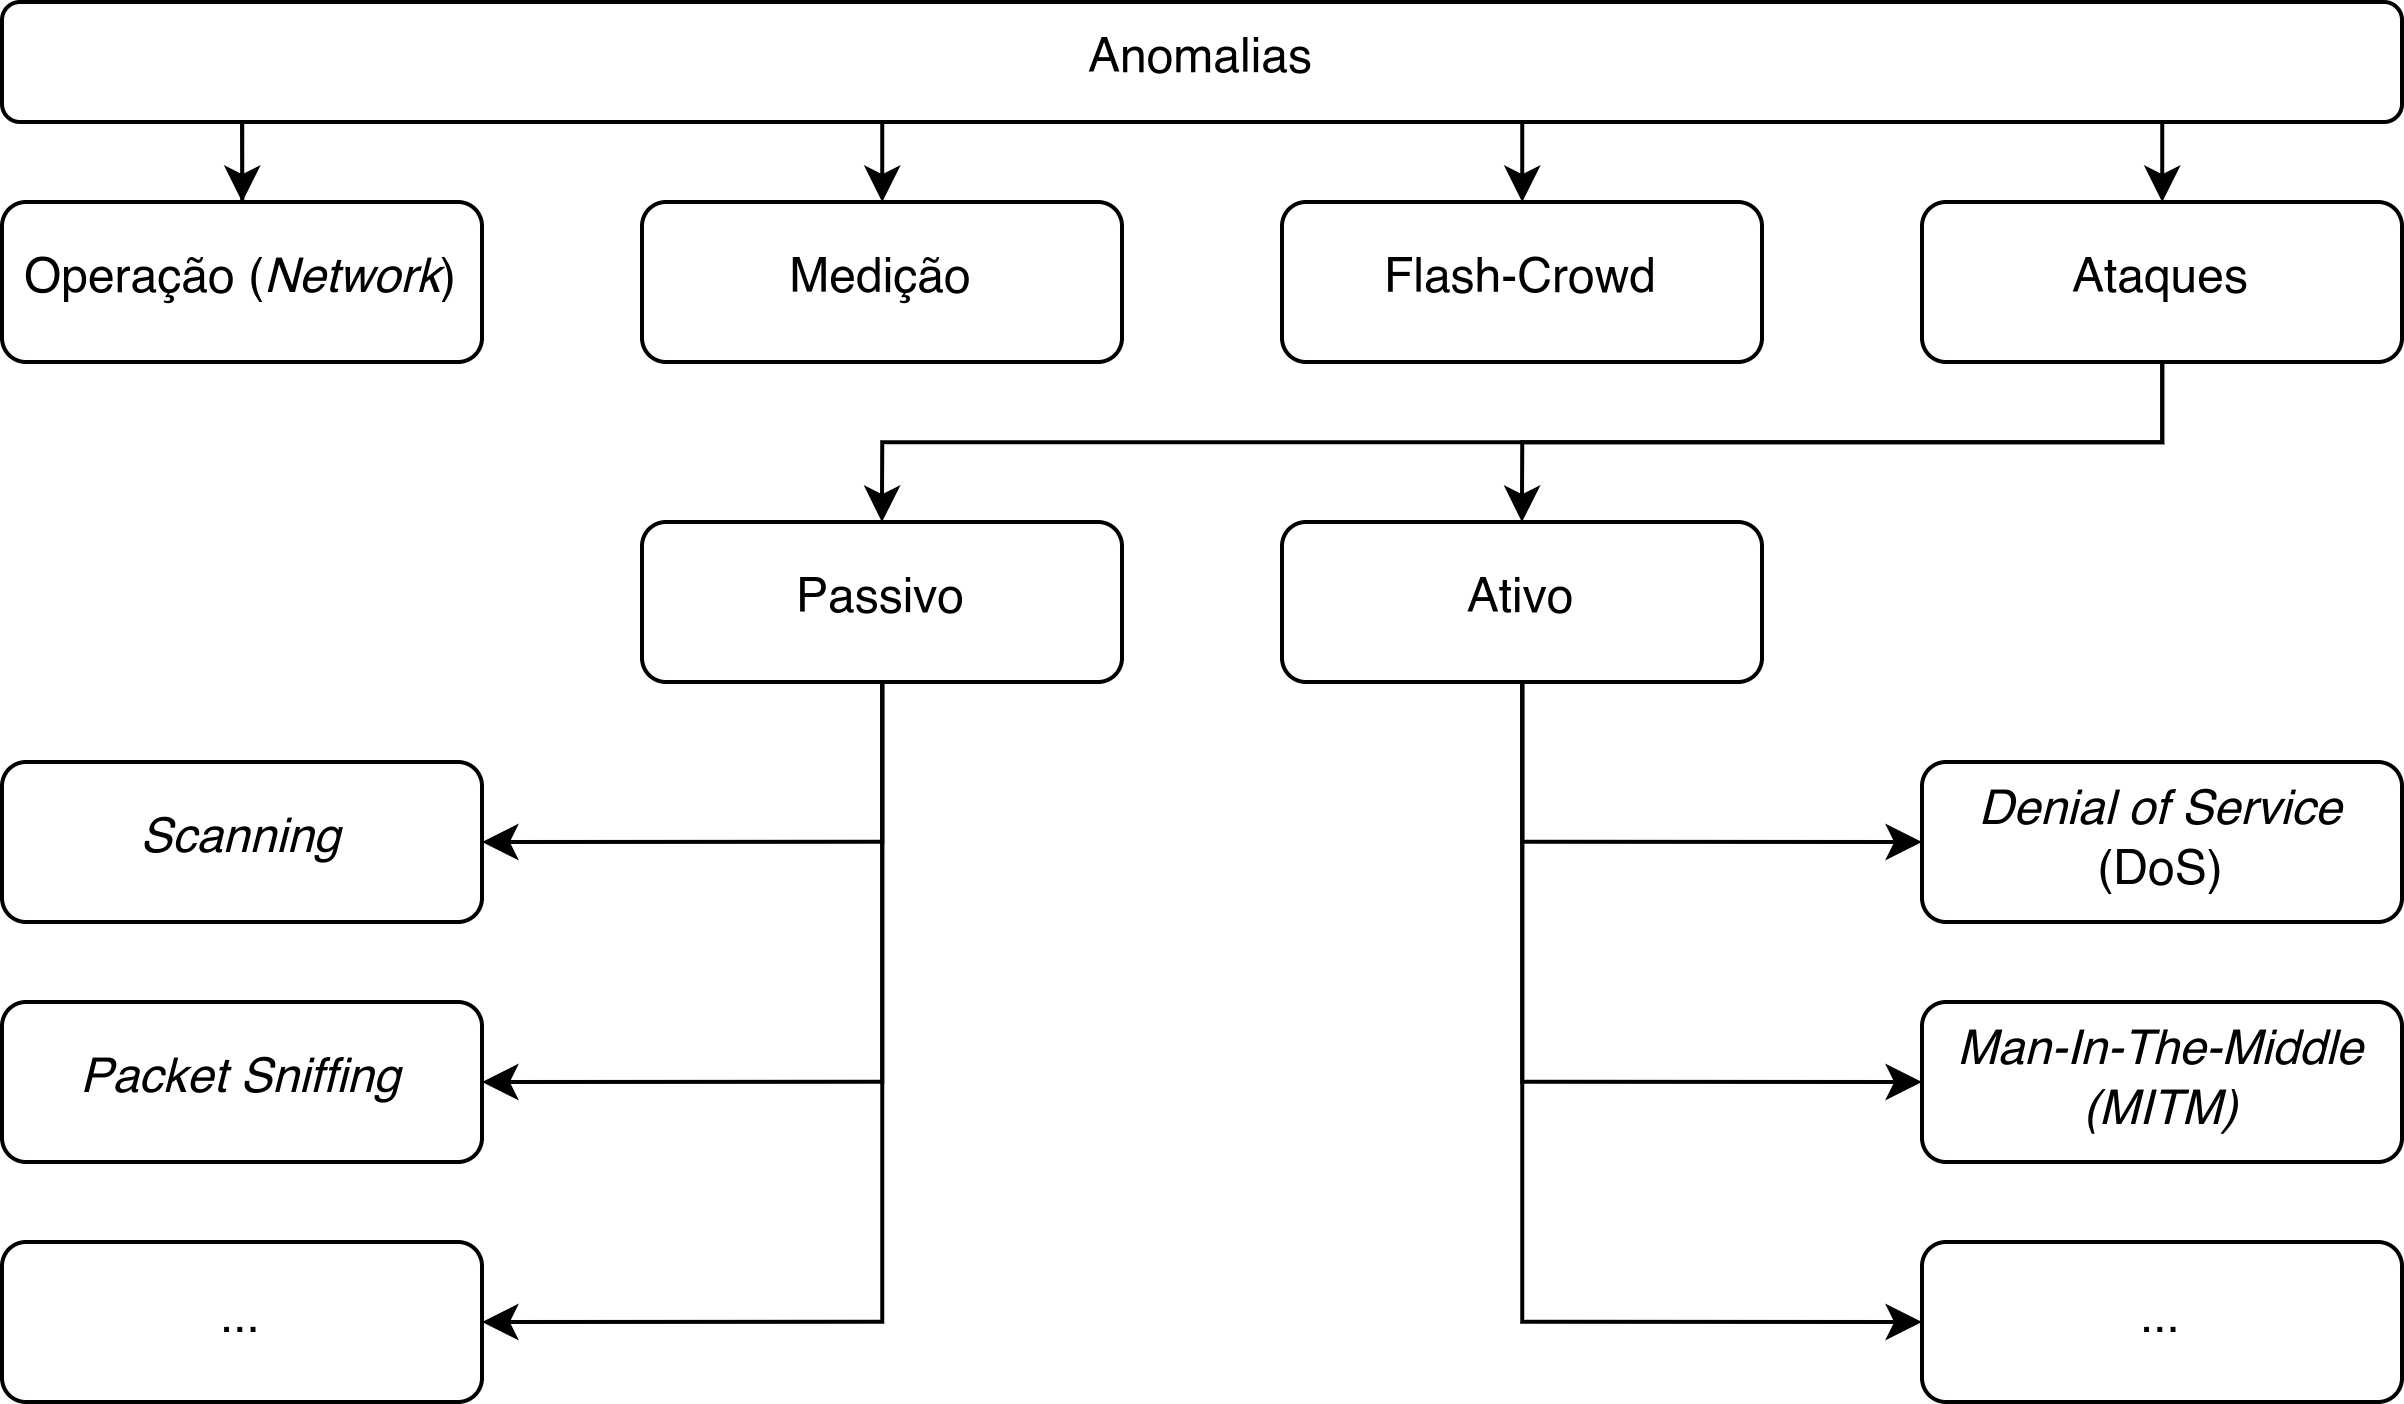
\includegraphics[height=.85\textheight]{anomalies.png}
        \end{figure}
    \end{frame}

    \begin{frame}{Análise e descoberta de vulnerabilidades}
        \begin{columns}
            \begin{column}{.5\textwidth}
                \textbf{Análise de vulnerabilidade no âmbito de \textit{software}:}
                \begin{wideitemize}
                    \item Estática
                    \item Dinâmica
                    \item Híbrida
                \end{wideitemize}
            \end{column}
            \begin{column}{.5\textwidth}
                \textbf{Descoberta de vulnerabilidades:}
                \begin{wideitemize}
                    \item Teste de Penetração
                    \item \textit{Fuzz-Testing}
                    \item Análise Estática de Fluxo de Dados
                \end{wideitemize}
            \end{column}
        \end{columns}
        \begin{figure}
            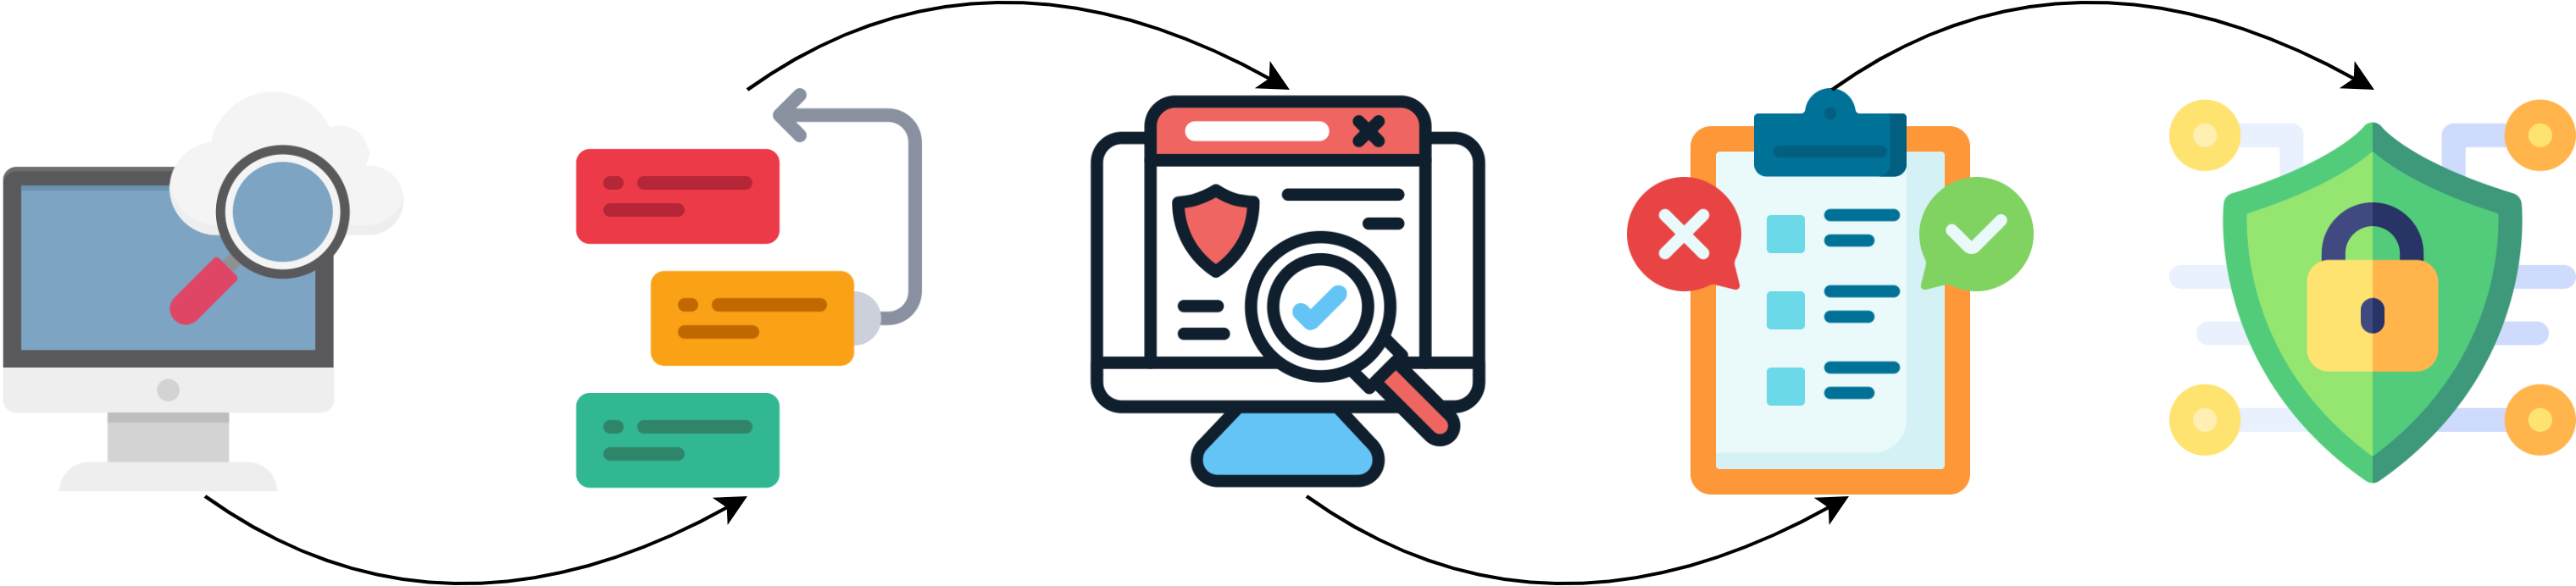
\includegraphics[width=.8\textwidth]{vulAnalysis.png}
        \end{figure}
    \end{frame}

    \section{Desenvolvimento}
    \subsection{Bancada Experimental}

    \begin{frame}{Bancada experimental}{para testes de intrusões em redes OPC UA}
        \begin{columns}
            \begin{column}{.6\textwidth}
                \begin{figure}
                    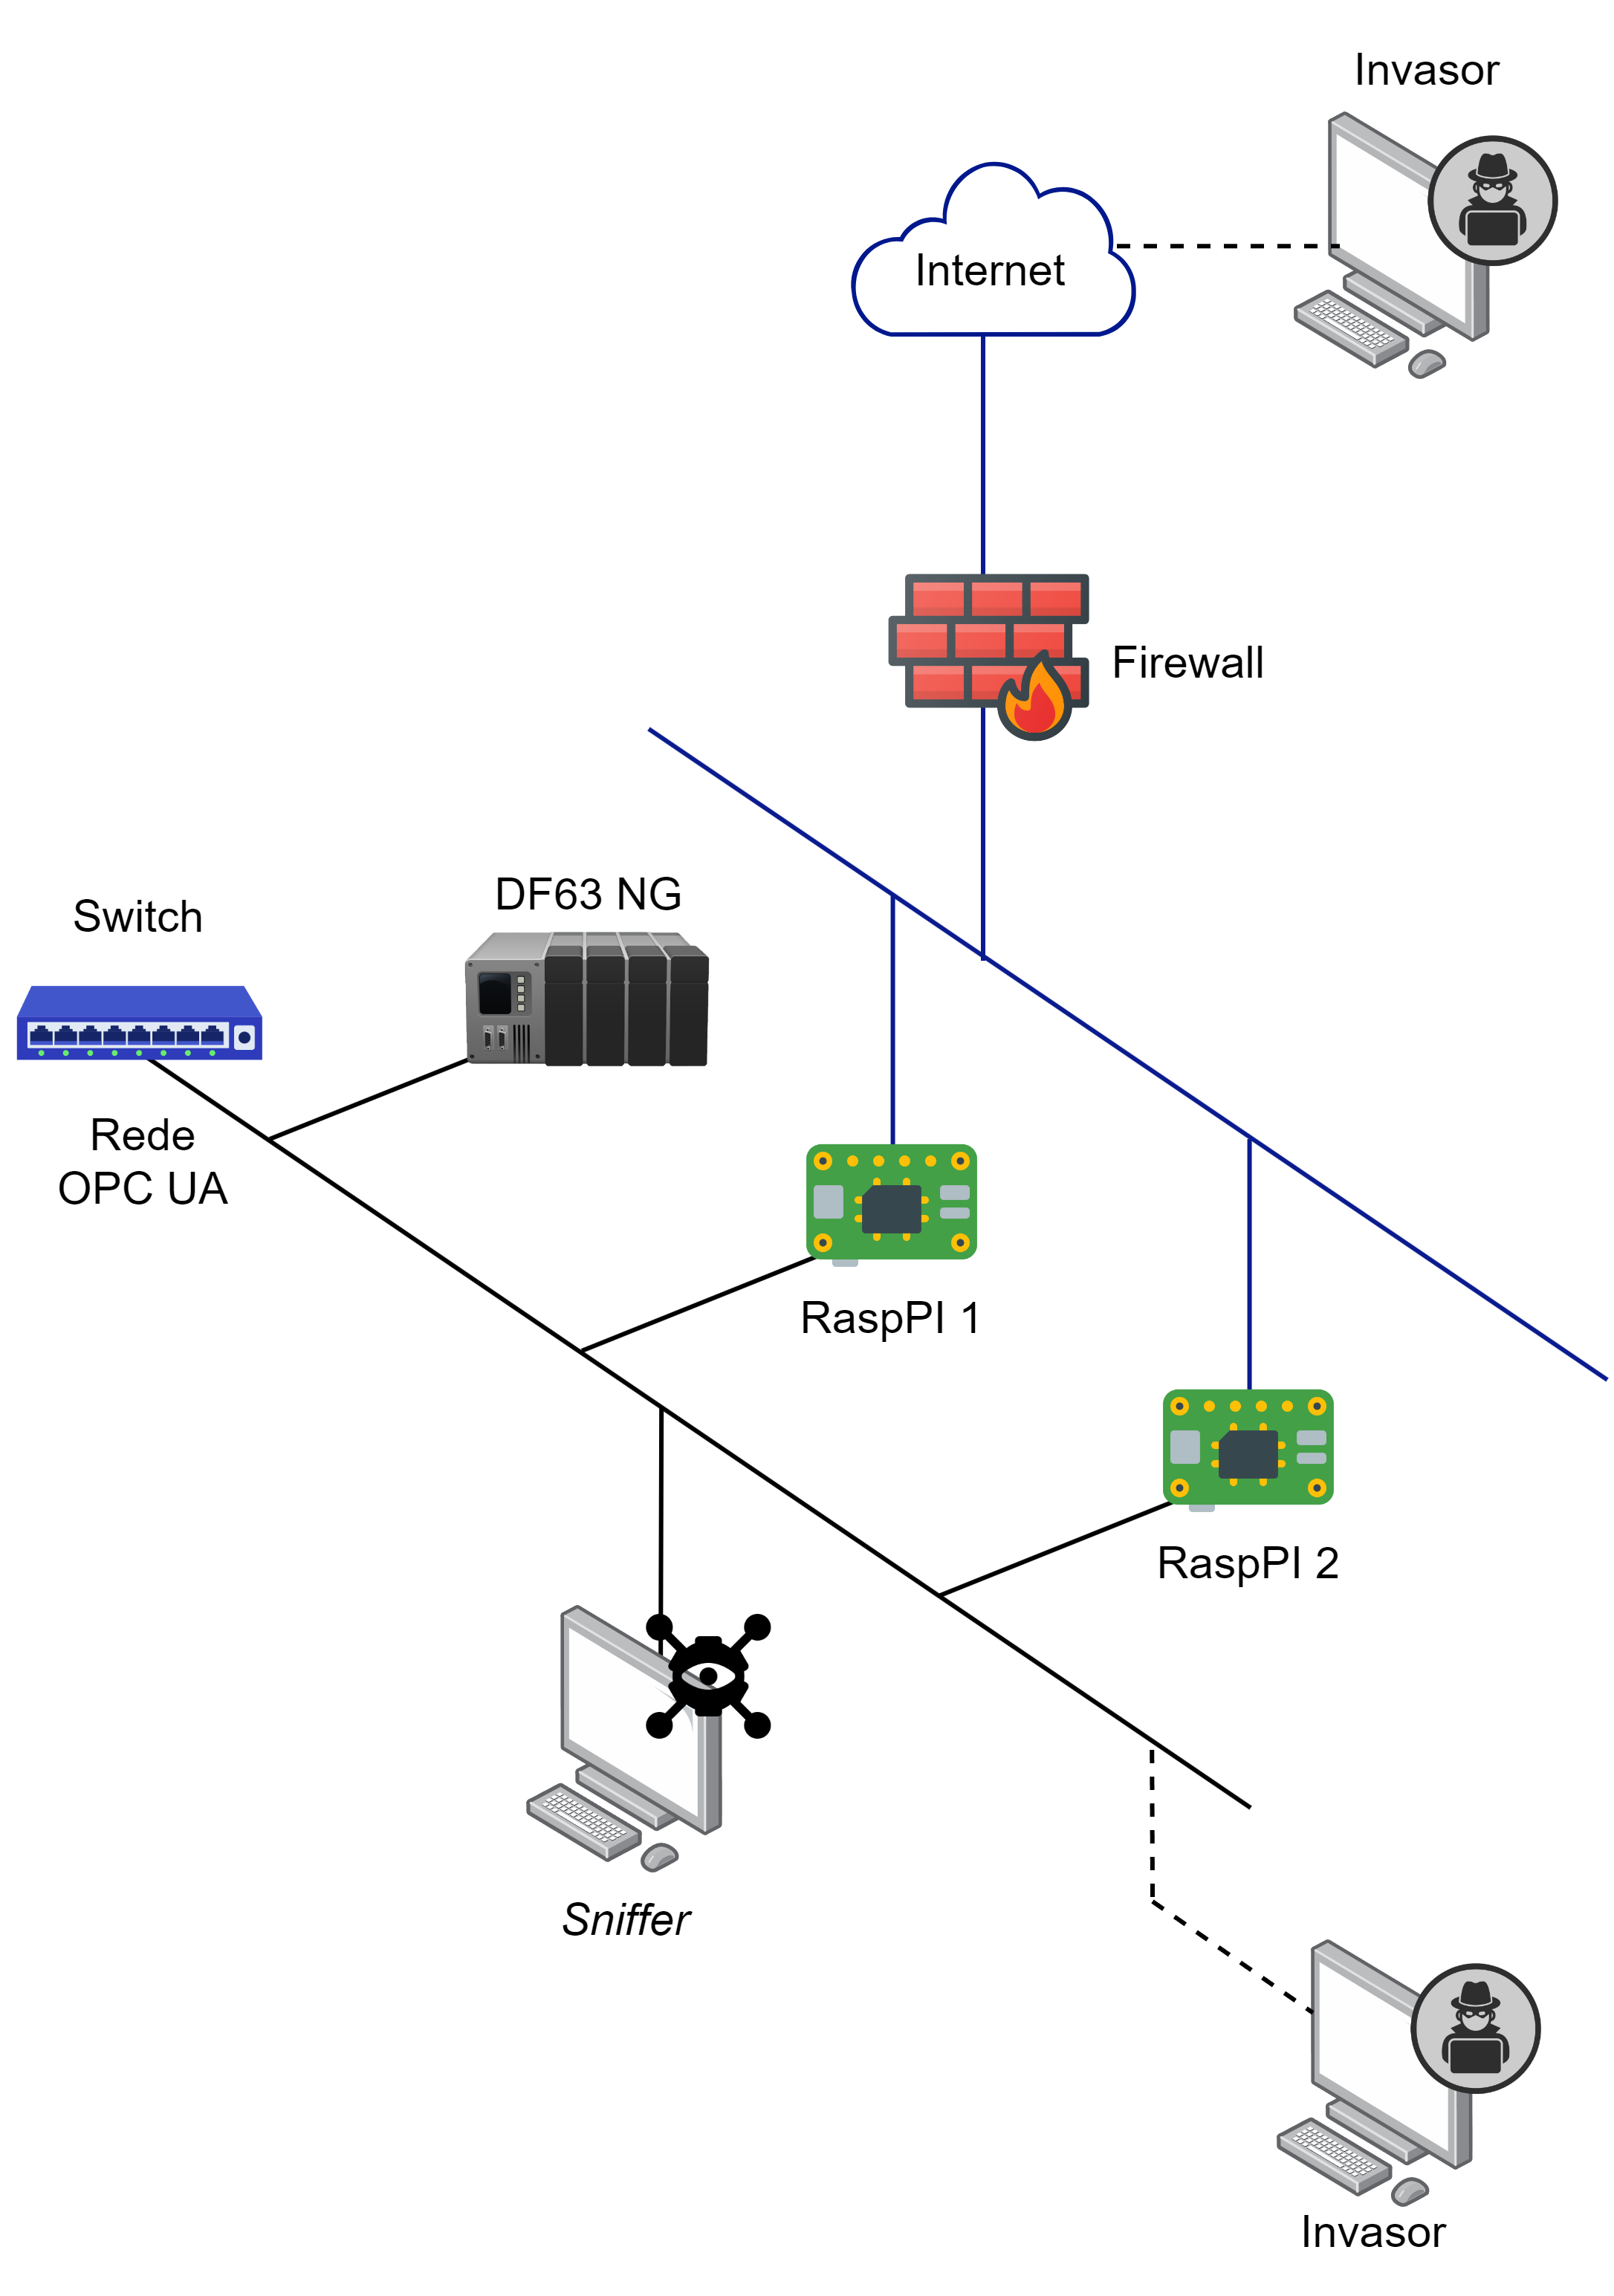
\includegraphics[height=0.8\textheight]{bancada.png}
                \end{figure}
            \end{column}
            \begin{column}{.4\textwidth}
                \only<1>{
                    \textit{\textbf{Hardware}}
                    \begin{wideitemize}
                        \item DF63 NG
                        \item Raspberry Pi 4 Modelo B
                        \item Ethernet Switch
                        \item Elemento Invasor
                    \end{wideitemize}
                }
                \only<2>{
                    \textit{\textbf{Software}}
                    \begin{wideitemize}
                        \item Smar OPC UA server
                        \item opcua-asyncio
                        \item OPC UA Exploit Framework
                        \item Ettercap
                        \item Hping3
                        \item Wireshark
                        \item Nmap
                    \end{wideitemize}
                }
                \only<3>{
                    \begin{figure}
                        \includegraphics[height=0.8\textheight]{cyberkit2.png}
                    \end{figure}
                }
            \end{column}
        \end{columns}
    \end{frame}

    \subsection{Ataques em Redes Industriais OPC UA}

    \begin{frame}{\textit{Packet Sniffing}}
        \begin{columns}
            \begin{column}{.5\textwidth}
                \begin{wideitemize}
                    \item Monitorar comunicação OPC UA
                    \item Roubar dados sigilosos (caso rede OPC UA não seja configurada corretamente)
                    \item Ataque de entrada para outros
                \end{wideitemize}
            \end{column}
            \begin{column}{.5\textwidth}
                \textbf{Execução:}
                \begin{wideitemize}
                    \item Ettercap
                    \item Wireshark
                \end{wideitemize}
            \end{column}
        \end{columns}
        \begin{figure}
            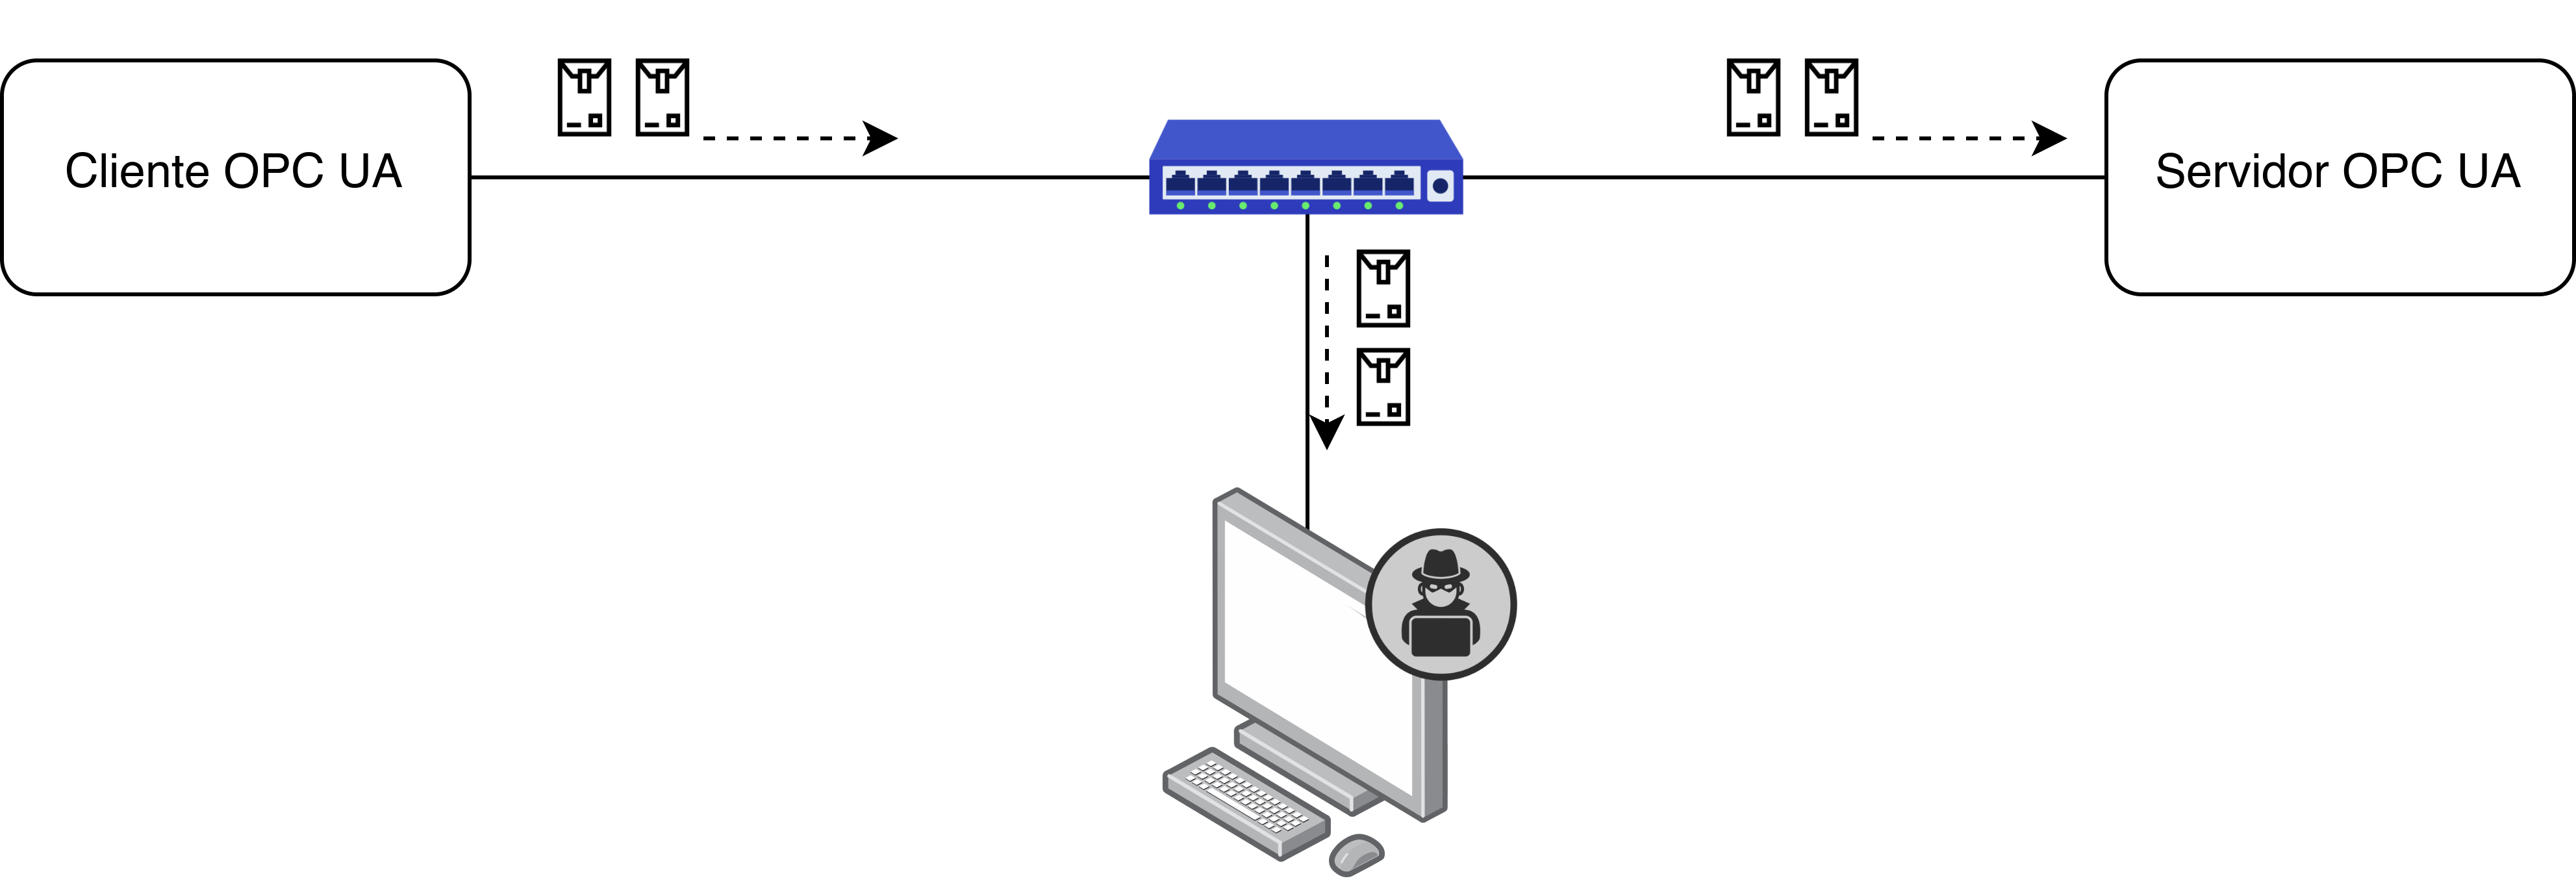
\includegraphics[width=.7\textwidth]{sniffing.png}
        \end{figure}
    \end{frame}

    \begin{frame}{\textit{Man-in-The-Middle (MITM)}}
        \begin{columns}
            \begin{column}{.5\textwidth}
                \begin{wideitemize}
                    \item Interceptação das informações do \textit{SecureChannel}
                    \item Inserção de elementos não confiáveis na rede OPC UA ao trocar os endereços MAC, pelo ARP \textit{Spoofing}
                    \item Concede ao Elemento Invasor o poder de visualizar e/ou alterar informações da comunicação
                \end{wideitemize}
            \end{column}
            \begin{column}{.5\textwidth}
                \textbf{Execução:}
                \begin{wideitemize}
                    \item Ettercap
                    \item Wireshark
                \end{wideitemize}
            \end{column}
        \end{columns}
        \begin{figure}
            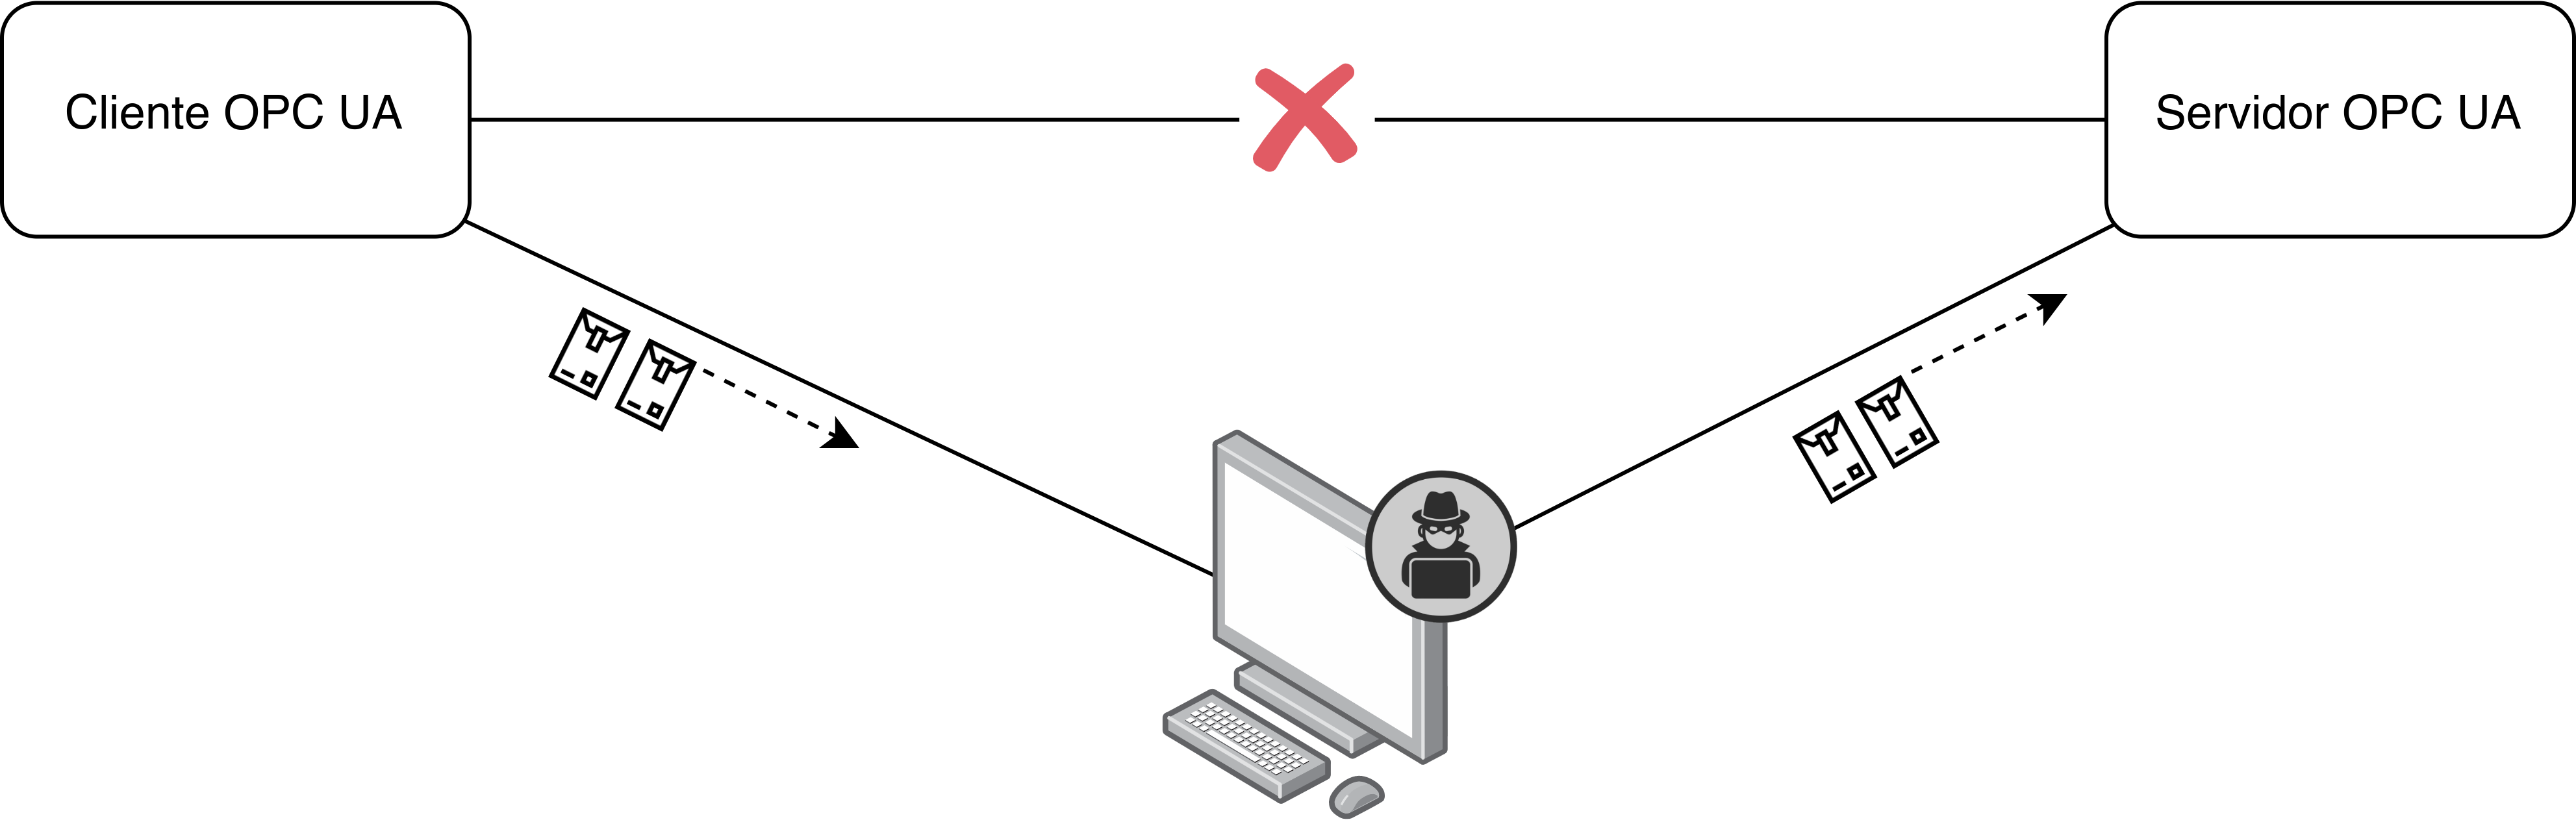
\includegraphics[width=.7\textwidth]{mitm.png}
        \end{figure}
    \end{frame}

    \begin{frame}{\textit{Denial of Service (DoS)}}
        \only<1>{
            \begin{columns}
                \begin{column}{.6\textwidth}
                    \begin{wideitemize}
                        \item Inundação da rede e do servidor ao enviar mensagens específicas continuamente
                        \item Concede ao Elemento Invasor o poder de visualizar e/ou alterar informações da comunicação
                    \end{wideitemize}
                \end{column}
                \begin{column}{.4\textwidth}
                    \textbf{Execução:}
                    \begin{itemize}
                        \item Nmap
                        \item OPC UA Exploit Framework
                        \item Hping3
                        \item Wireshark
                    \end{itemize}
                \end{column}
            \end{columns}
            \begin{figure}
                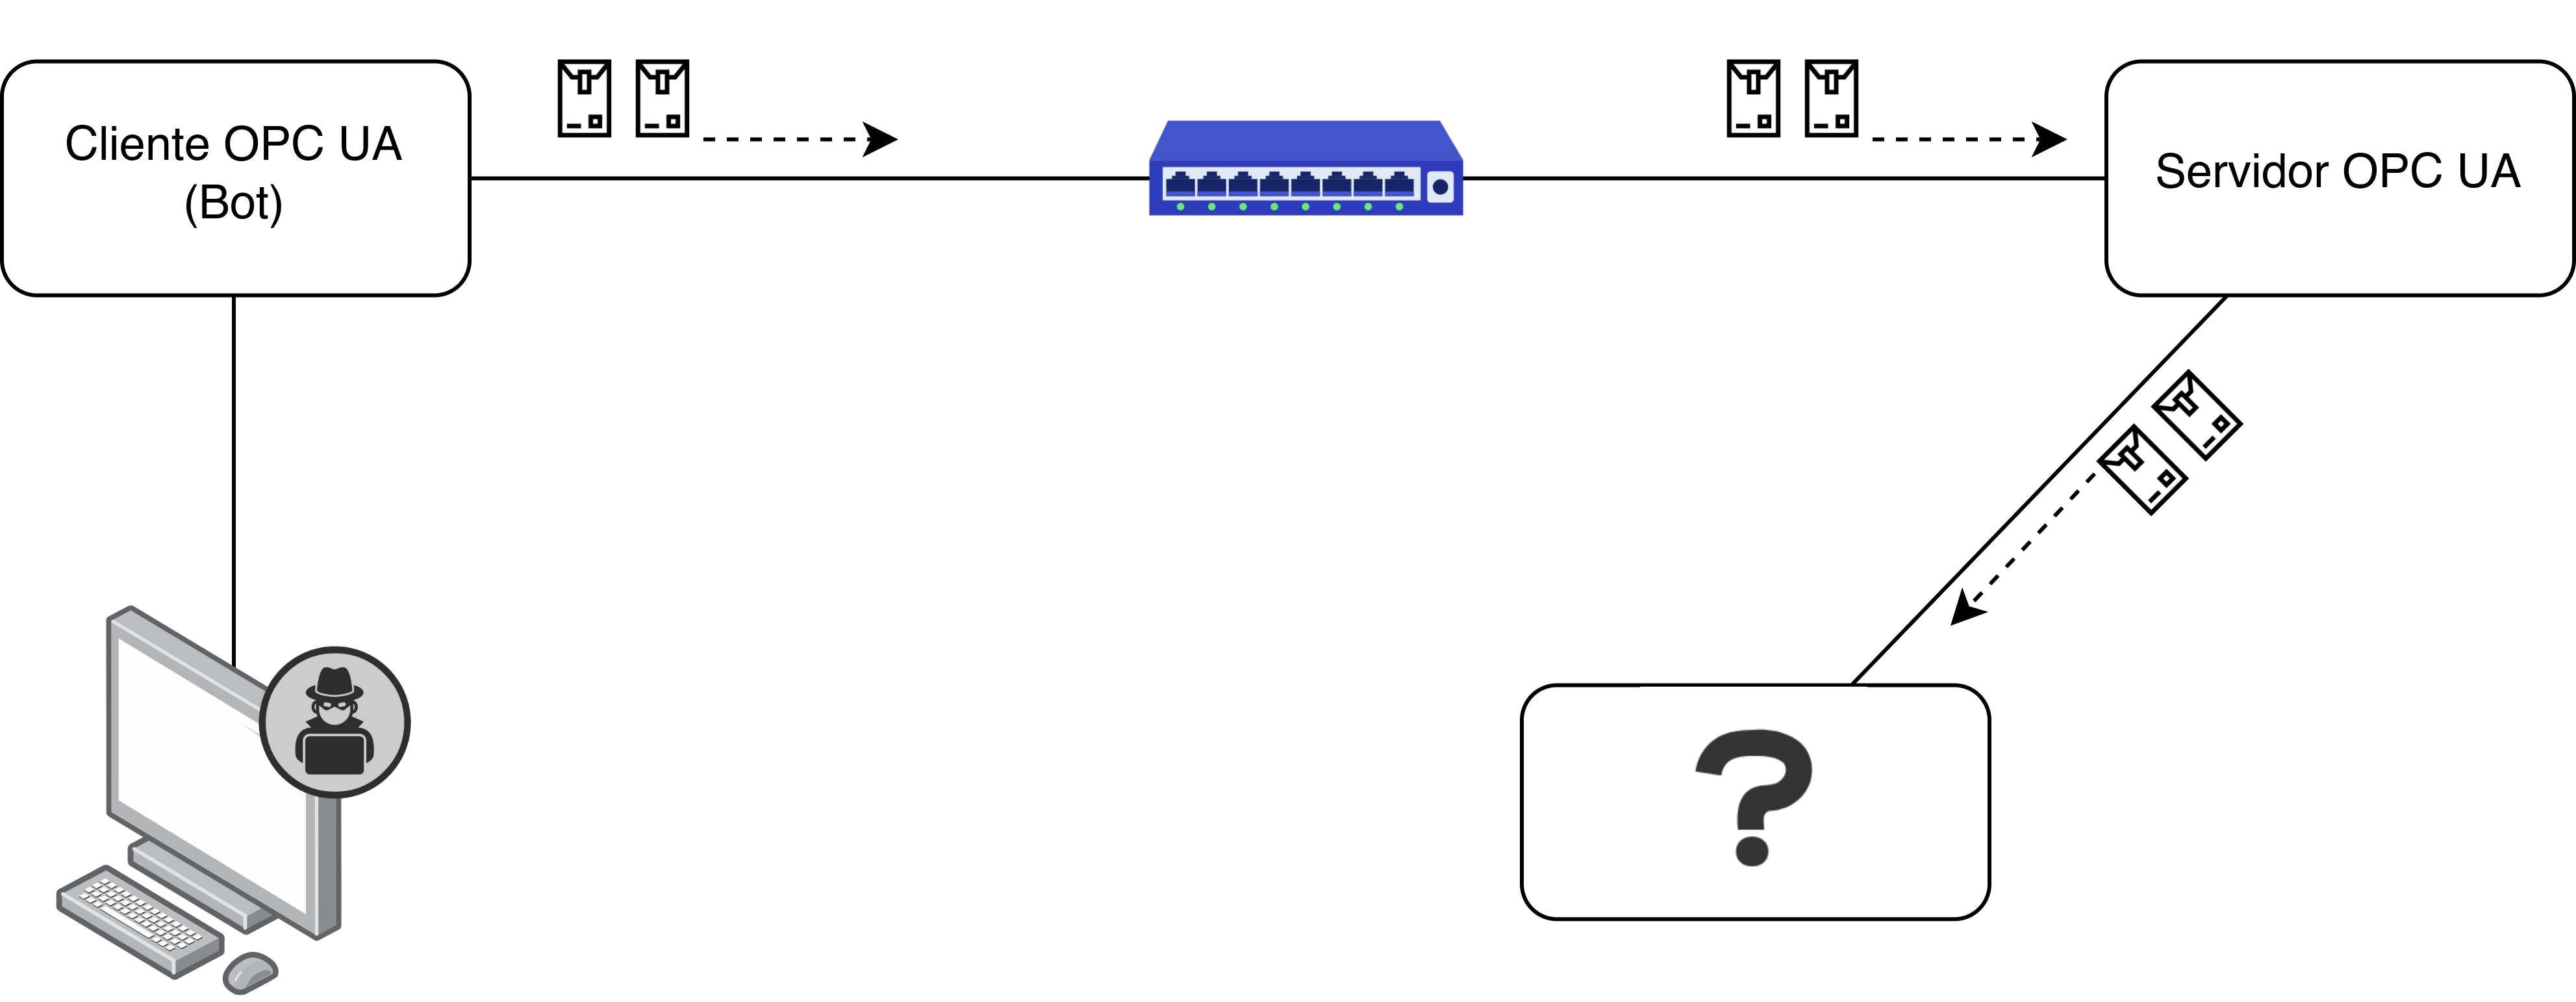
\includegraphics[width=.7\textwidth]{dos.png}
            \end{figure}
        }
        \only<2>{
            \begin{columns}
                \begin{column}{.6\textwidth}
                    \textbf{SYN Flooding:}
                    \begin{wideitemize}
                        \item Utilização do Nmap para a varredura da rede
                        \item Uma vez mapeada, aplica-se o Hping3 para realizar este ataque
                    \end{wideitemize}
                \end{column}
                \begin{column}{.4\textwidth}
                    \begin{figure}
                        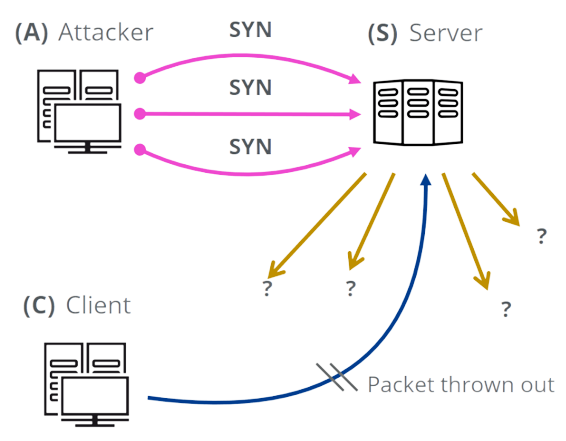
\includegraphics[width=.7\textwidth]{syn-flooding.png}
                    \end{figure}
                \end{column}
            \end{columns}
        }
        \only<3>{
            \begin{columns}
                \begin{column}{.6\textwidth}
                    \textbf{HEL Flooding:}
                    \begin{wideitemize}
                        \item No caso do OPC UA, envio de mensagens contínuas HEL (\textit{Hello message}) para o servidor
                        \item Endpoint URL: \textcolor{blue}{opc.tcp}://\textcolor{orange}{192.168.164.102}:\textcolor{green}{4840}/\textcolor{red}{opcua/}
                        \begin{itemize}
                            \item \textit{Scheme}: \textcolor{blue}{opc.tcp} ou \textcolor{blue}{opc.https}
                            \item \textcolor{orange}{Endereço do servidor}
                            \item \textcolor{green}{Porta}
                            \item \textcolor{red}{DircoveryEndpoint}
                        \end{itemize}
                    \end{wideitemize}
                \end{column}
                \begin{column}{.4\textwidth}
                    \begin{figure}
                        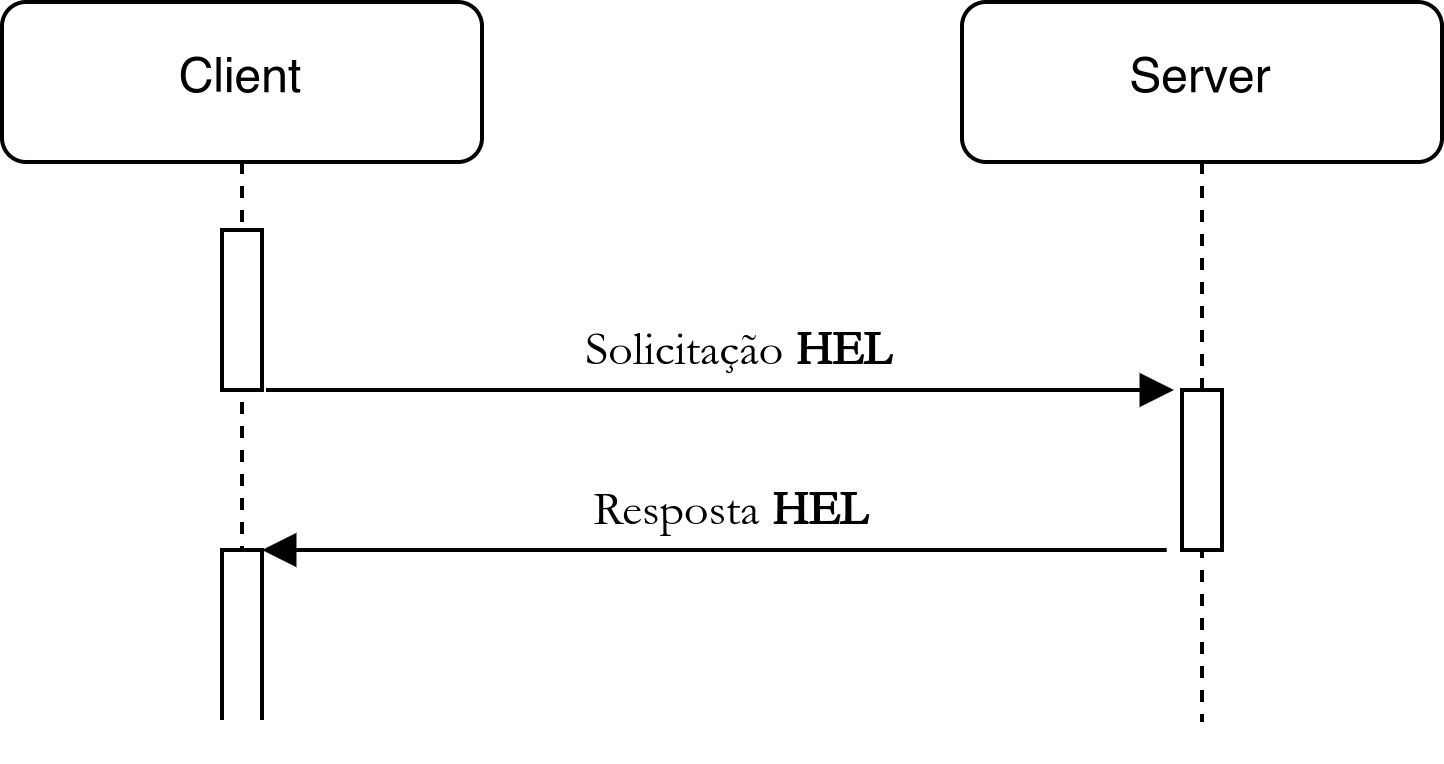
\includegraphics[width=.7\textwidth]{helMessage2.png}
                    \end{figure}
                \end{column}
            \end{columns}
            \begin{figure}
                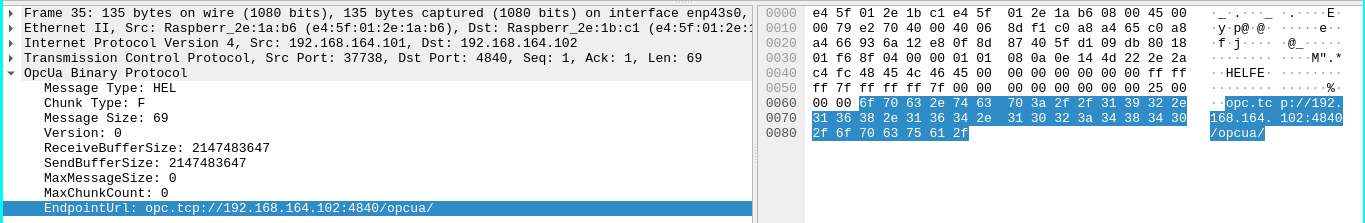
\includegraphics[width=.7\textwidth]{helMessage.png}
            \end{figure}
        }
        \only<4>{
            \begin{columns}
                \begin{column}{.6\textwidth}
                    \textbf{Chunk Flooding:}
                    \begin{wideitemize}
                        \item \textit{Chunk} refere-se a uma unidade de dados que pode ser transmitida entre um cliente e um servidor OPC UA
                        \item Caso ocorra um erro na criação de um destes fragmentos, um \textit{Chunk} final deve ser enviado
                        \item A inundação por \textit{Chunk} envolve o envio de uma quantidade abundante de fragmentos de dados ao servidor sem o envio do fragmento final correspondente
                    \end{wideitemize}
                \end{column}
                \begin{column}{.4\textwidth}
                    \begin{figure}
                        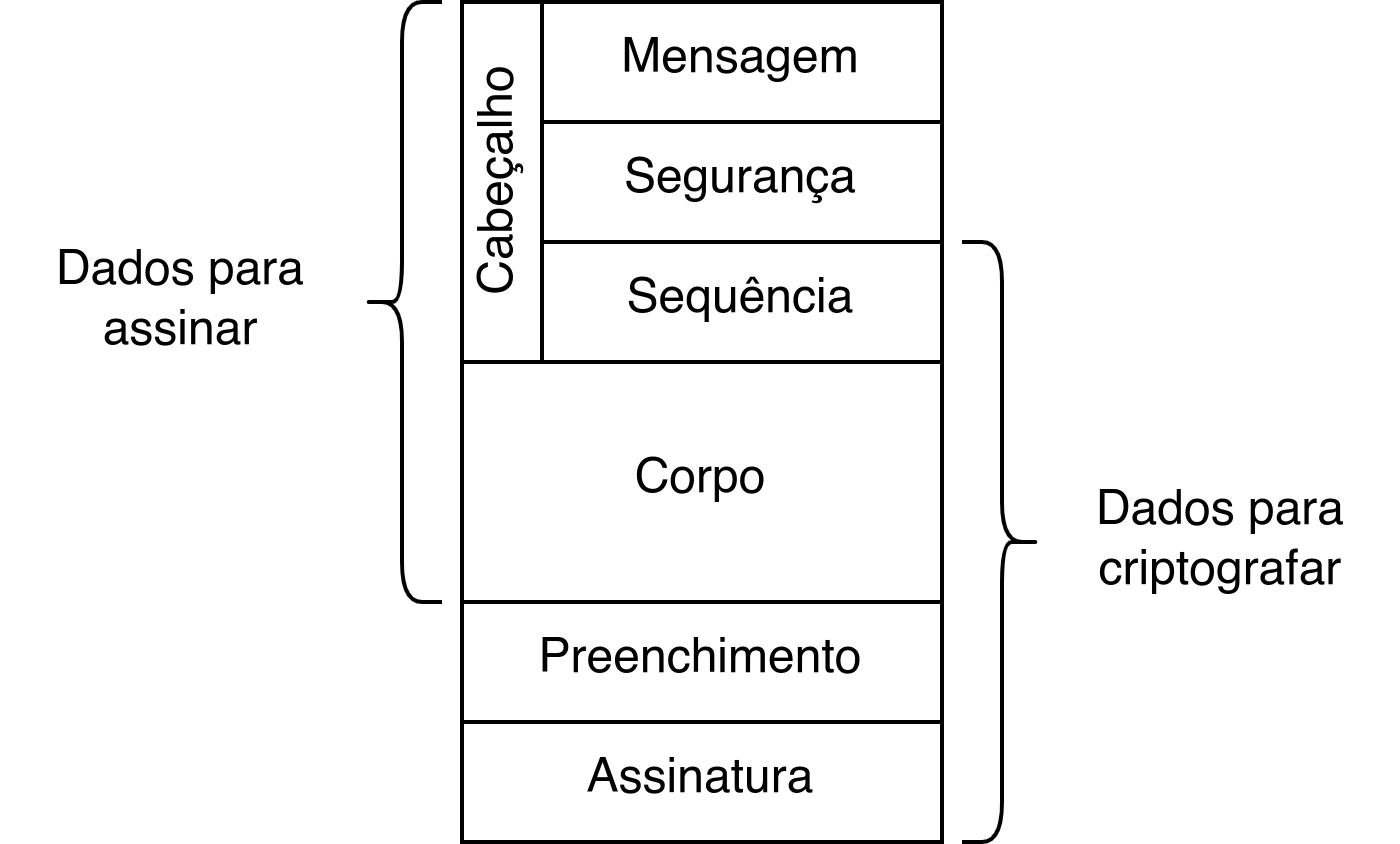
\includegraphics[width=.8\textwidth]{chunk.png}
                    \end{figure}
                    \footnotetext{\href{https://reference.opcfoundation.org/Core/Part6/v104/docs/6.7}{MessageChunk de conversa segura OPC UA}}
                \end{column}
            \end{columns}
        }
        \only<5>{
            \begin{columns}
                \begin{column}{.6\textwidth}
                    \textbf{Abertura de múltiplos canais seguros:}
                    \begin{itemize}
                        \item Solicitações OPN (OpenSecureChannel) são enviadas continuamente ao servidor. 
                        \item Recursos substanciais são consumidos durante a validação do certificado, na solicitação e no processo de criptografia da mensagem
                        \item Pode ser ainda mais eficaz quando a Autoridade de Certificação está localizada em um sistema diferente
                    \end{itemize}
                \end{column}
                \begin{column}{.4\textwidth}
                    \begin{figure}
                        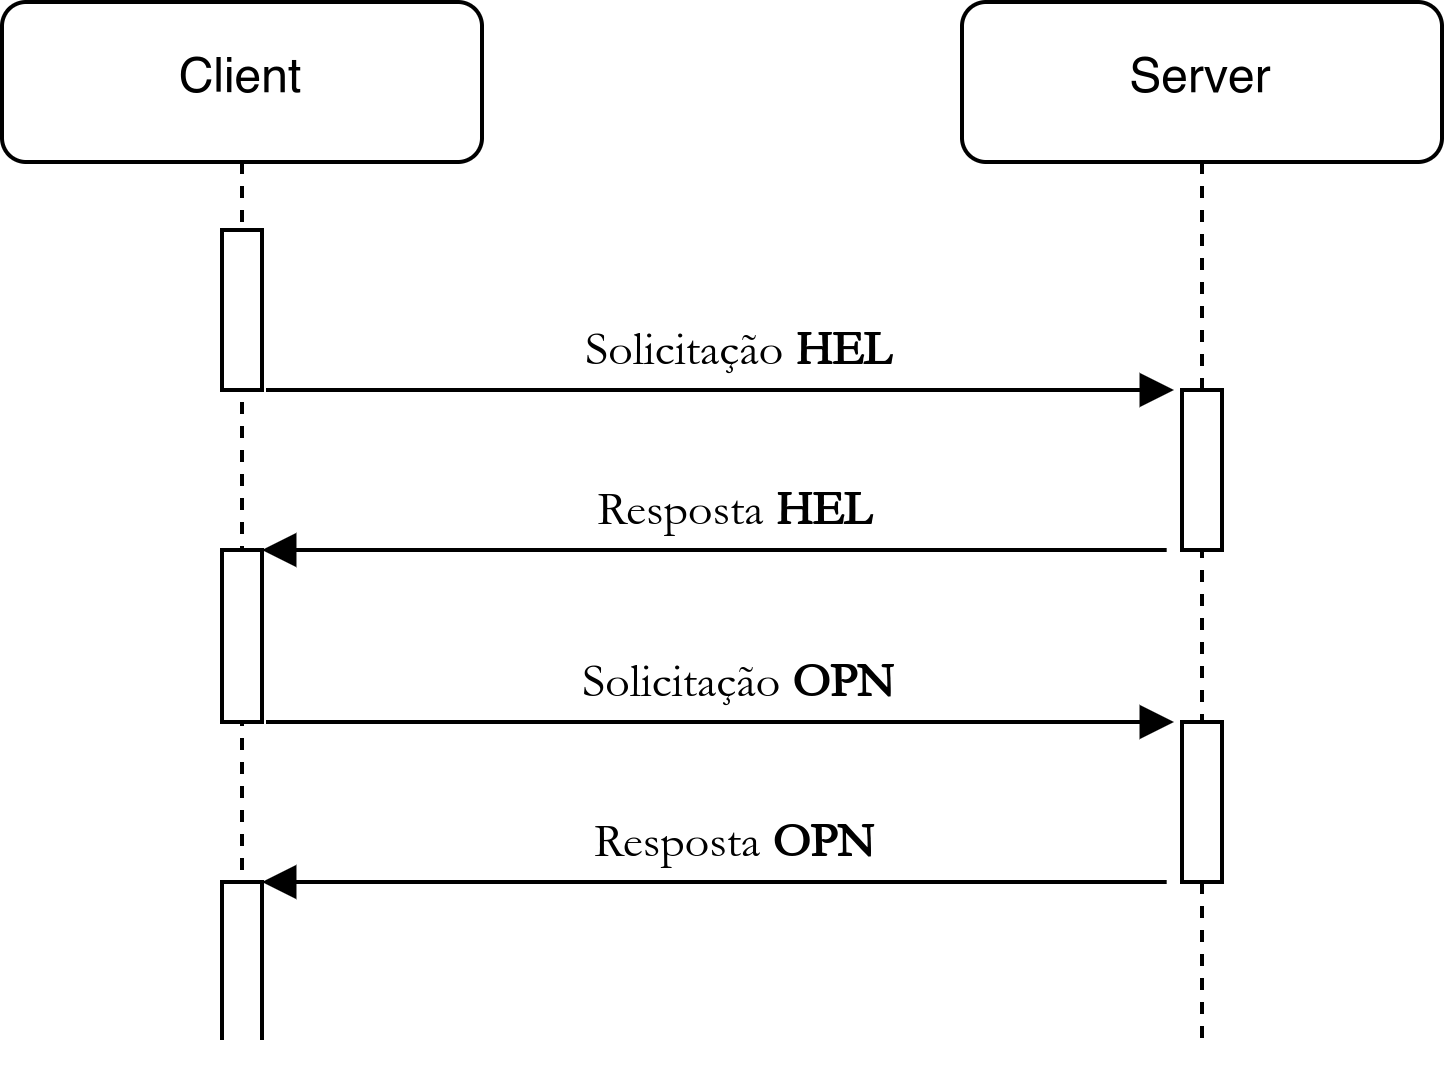
\includegraphics[width=.7\textwidth]{opn.png}
                    \end{figure}
                \end{column}
            \end{columns}
            \begin{figure}
                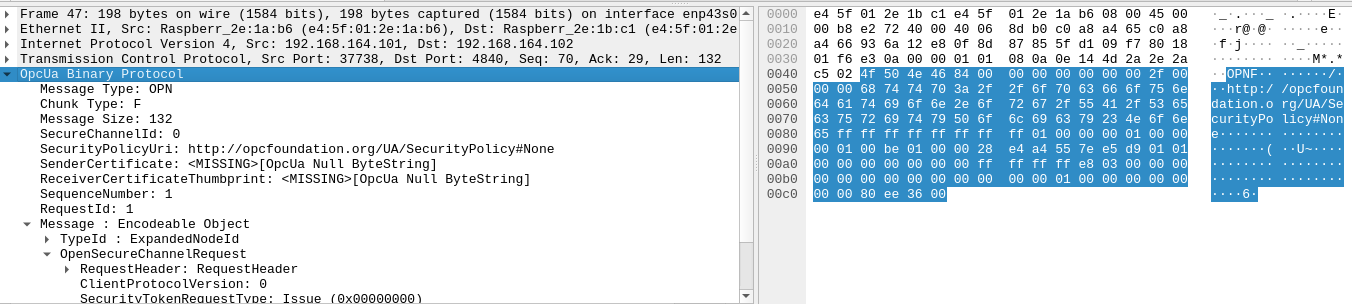
\includegraphics[width=.7\textwidth]{wireshark-opn.png}
            \end{figure}
        }
        \only<6>{
            \begin{columns}
                \begin{column}{.6\textwidth}
                    \textbf{Tradução do caminho de navegação:}
                    \begin{wideitemize}
                        \item São enviadas ao servidor requisições de traduções de \textit{browse path} complexas que exploram a falta de limites adequados na resolução destes caminhos
                    \end{wideitemize}
                \end{column}
                \begin{column}{.4\textwidth}
                    \begin{figure}
                        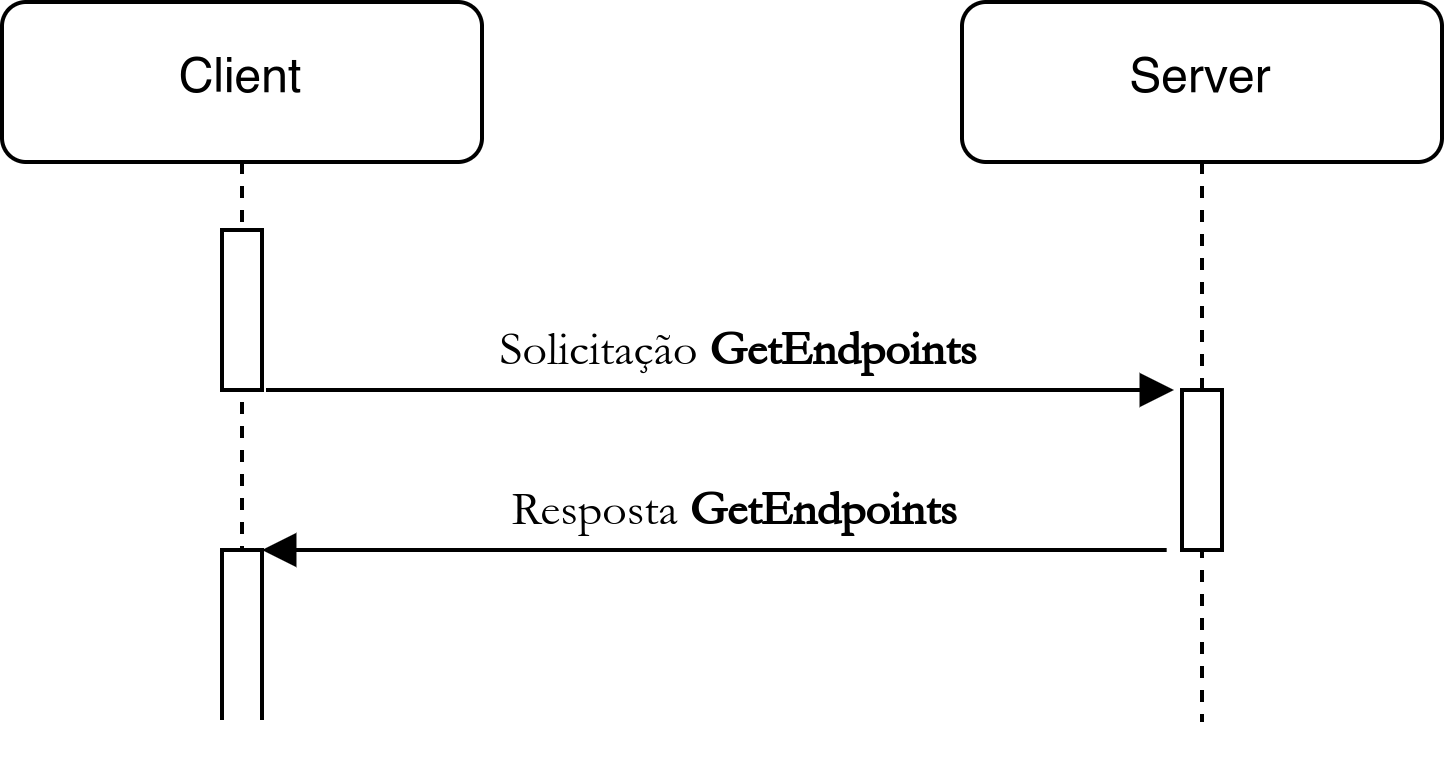
\includegraphics[width=.7\textwidth]{getEndpoints.png}
                    \end{figure}
                \end{column}
            \end{columns}
        }
    \end{frame}

    \subsection{Metodologia}

    \begin{frame}{Fluxo de atividades}
        \begin{figure}
            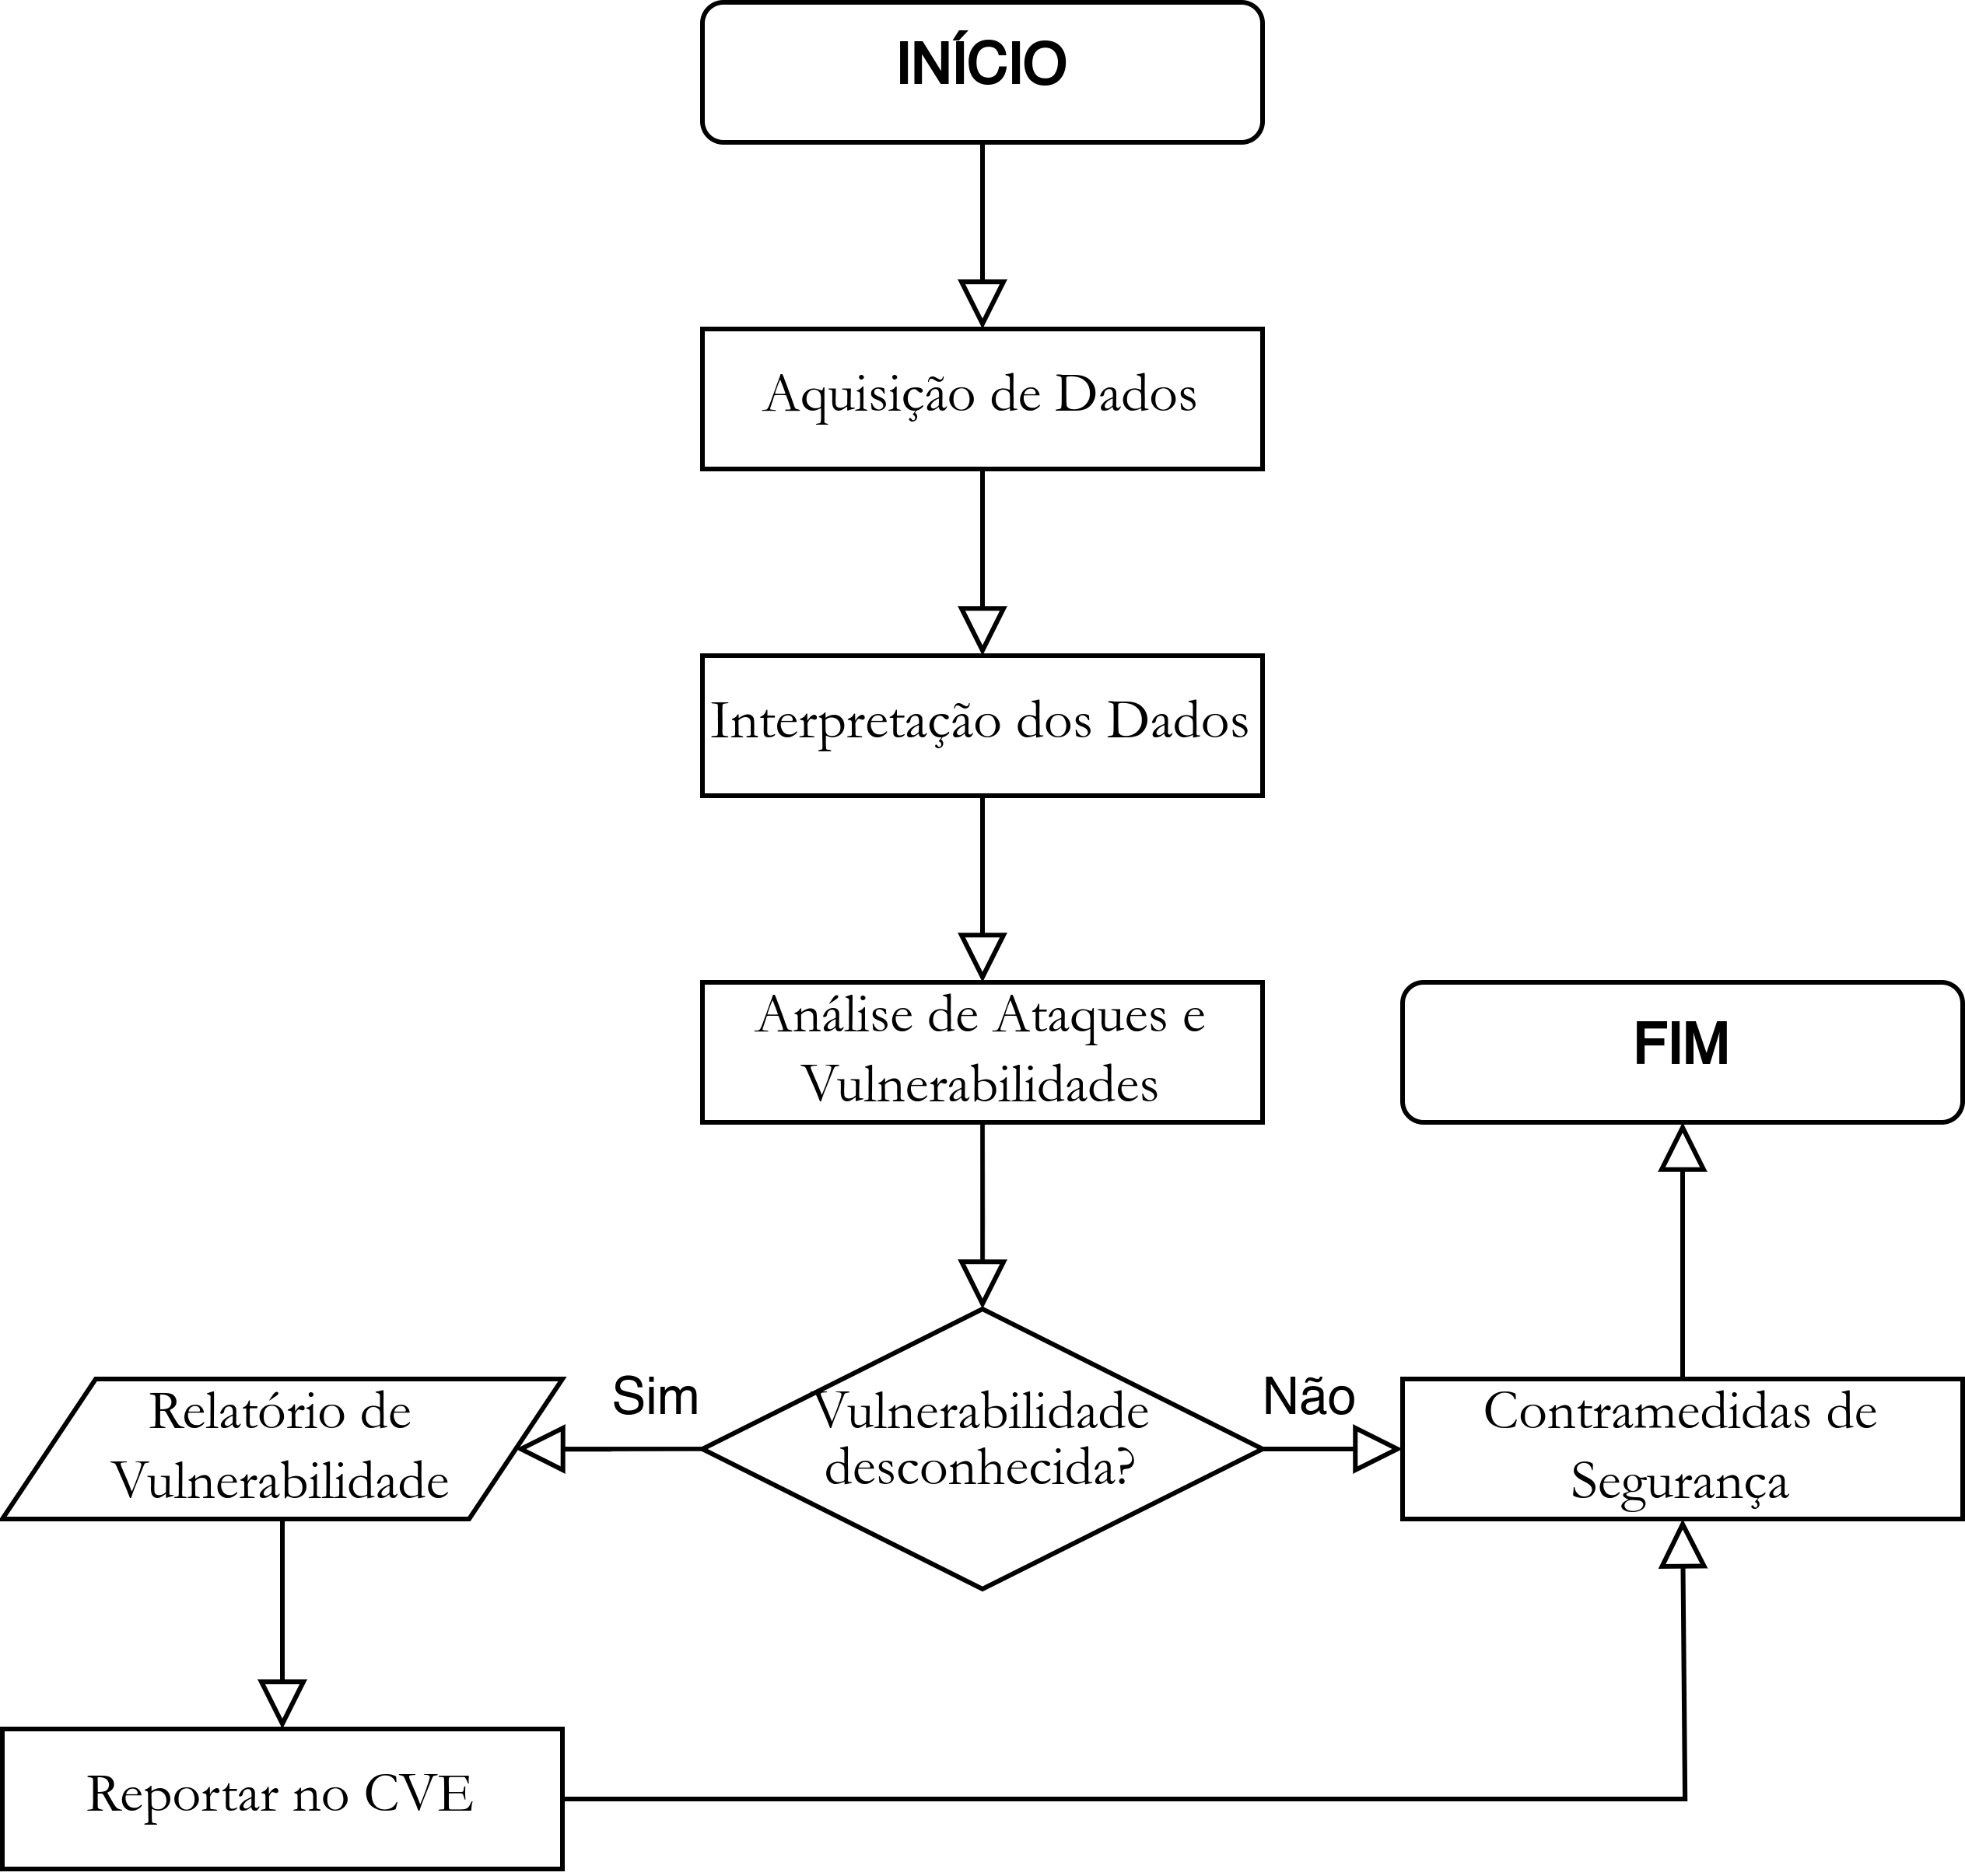
\includegraphics[height=.83\textheight]{fluxograma.png}
        \end{figure}
    \end{frame}

    \section{Resultados Esperados}

    \begin{frame}
        \begin{columns}[t]
            \begin{column}{.33\textwidth}
                \textbf{Sniffing:}
                \begin{wideitemize}
                    \item Alto nível de resistência à interceptação não autorizada de pacotes, dependendo do nível de segurança aplicado
                    \item Segurança garantida no modo Sign\&Encrypt
                    \item Comprometimento da confidencialidade dos dados nos demais modos de segurança
                \end{wideitemize}
            \end{column}
            \begin{column}{.33\textwidth}
                \textbf{MITM:}
                \begin{wideitemize}
                    \item Dependência significativa da configuração aplicada na comunicação
                    \item Caso nível mais alto de segurança, o OPC UA não deve permitir a quebra de algum pilar de segurança
                    \item No entanto, a integridade dos dados pode ser comprometida nos demais níveis
                    \item Contramedidas devem ser propostas para as falhas encontradas 
                \end{wideitemize}
            \end{column}
            \begin{column}{.33\textwidth}
                \textbf{DoS:}
                \begin{wideitemize}
                    \item Depende da capacidade da rede e do processamento dos hospedeiros
                    \item Em redes reais, os efeitos devem ser potencializados devido à quantidade de equipamentos
                    \item Esgotamento de recursos em alguns tipos de ataques de negação de serviço, comprometendo disponibilidade dos dados
                \end{wideitemize}
            \end{column}
        \end{columns}
    \end{frame}

    \section{Metas estabelecidas}
    \begin{frame}
        \begin{table}[H]
            \caption{Metas estabelecidas para a projeto.}
            \label{tab:metas}
            \centering
            \begin{tabular}{
                |>{\centering\arraybackslash}m{0.075\textwidth}
                |>{\raggedright\arraybackslash}m{0.88\textwidth}
            |} \hline
                \textbf{Metas} & \multicolumn{1}{c|}{\textbf{Descrição}} \\ \hline
                1 & Pesquisa bibliográfica \\ \hline
                2 & Projeto e implementação do ambiente de teste para coleta de dados \\ \hline
                3 & Análise e escolha dos ataques cibernéticos \\ \hline
                4 & Implementação dos ataques na bancada experimental \\ \hline
                5 & Dissertação para exame de qualificação \\ \hline
                6 & Coleta e interpretação dos dados \\ \hline
                7 & Análise dos ataques e vulnerabilidades em redes industriais OPC UA \\ \hline
                8 & Verificação de desempenho e validação dos resultados \\ \hline
                9 & Escrita e submissão de artigo científico \\ \hline
                10 & Entrega final e defesa da dissertação \\
                \hline
            \end{tabular}
        \end{table}
    \end{frame}

    \subsection{Cronograma proposto}
    \begin{frame}
        \begin{table}[H]
            \centering
            \caption{Cronograma proposto para cumprimento das metas.}
            \label{tab:cronograma}
            \begin{tabular}{
                |>{\centering\arraybackslash}m{0.075\textwidth}
                |>{\centering\arraybackslash}m{0.065\textwidth}
                |>{\centering\arraybackslash}m{0.04\textwidth}
                |>{\centering\arraybackslash}m{0.04\textwidth}
                |>{\centering\arraybackslash}m{0.04\textwidth}
                |>{\centering\arraybackslash}m{0.04\textwidth}
                |>{\centering\arraybackslash}m{0.04\textwidth}
                |>{\centering\arraybackslash}m{0.04\textwidth}
                |>{\centering\arraybackslash}m{0.04\textwidth}
                |>{\centering\arraybackslash}m{0.04\textwidth}
                |>{\centering\arraybackslash}m{0.04\textwidth}
                |>{\centering\arraybackslash}m{0.04\textwidth}
                |>{\centering\arraybackslash}m{0.04\textwidth}
                |>{\centering\arraybackslash}m{0.04\textwidth}
                |>{\centering\arraybackslash}m{0.04\textwidth}
                |>{\centering\arraybackslash}m{0.04\textwidth}
                |>{\centering\arraybackslash}m{0.04\textwidth}
                |>{\centering\arraybackslash}m{0.04\textwidth}
            |} \hline
                \multicolumn{1}{|l|}{} & \textbf{2022} & \multicolumn{10}{c|}{\textbf{2023}} & \multicolumn{6}{c|}{\textbf{2024}} \\ \hline
                \textbf{Metas} & --         & 03 & 04 & 05 & 06 & 07 & 08 & 09 & 10 & 11 & 12 & 01 & 02 & 03 & 04 & 05 & 06 \\ \hline
                1    & \cellcolor{eescorange!30} & \y & \y & \y &    &    &    &    &    &    &    &    &    &    &    &    &    \\ \hhline{-~----------------}
                2    & \cellcolor{eescorange!30} &    & \y & \y & \y & \y & \y &    &    &    &    &    &    &    &    &    &    \\ \hhline{-~----------------}
                3    & \cellcolor{eescorange!30} &    &    &    & \y & \y & \y & \y &    &    &    &    &    &    &    &    &    \\ \hhline{-~----------------}
                4    & \cellcolor{eescorange!30} &    &    &    &    &    &    & \y & \x & \x & \x &    &    &    &    &    &    \\ \hhline{-~----------------}
                5    & \cellcolor{eescorange!30} &    &    &    &    & \y & \y & \y &    &    &    &    &    &    &    &    &    \\ \hhline{-~----------------}
                6    & \cellcolor{eescorange!30} &    &    &    &    &    &    &    & \x & \x & \x &    &    &    &    &    &    \\ \hhline{-~----------------}
                7    & \cellcolor{eescorange!30} &    &    &    &    &    &    &    &    &    &    & \x & \x &    &    &    &    \\ \hhline{-~----------------}
                8    & \cellcolor{eescorange!30} &    &    &    &    &    &    &    &    &    &    &    & \x & \x & \x &    &    \\ \hhline{-~----------------}
                9    & \cellcolor{eescorange!30} & \y & \y &    &    &    &    &    &    &    &    & \x & \x & \x &    &    &    \\ \hhline{-~----------------}
                10   & \cellcolor{eescorange!30}\multirow{-10}{*}{\rotatebox[origin=c]{90}{Disciplinas da pós-graduação}} &    &    &    &    &    &    &    &    &    &    &    &    &    &    & \x & \x \\ \hline
            \end{tabular}
            \begin{center}
                \textcolor{mainColor2}{$\blacksquare$} Itens realizados \hspace{1cm} \textcolor{mainColor1}{$\blacksquare$} Itens propostos
            \end{center}
        \end{table}
    \end{frame}

    %________________________________________________________
    %-------------------- REFERENCES ------------------------

    % \section*{References}
    \begin{frame}{Referências}
        \bibliographystyle{plain} % apalike
        \bibliography{references.bib}
    \end{frame}

    %________________________________________________________
    %-------------------- FINAL PAGE ------------------------

    {
        \usebackgroundtemplate{
\includegraphics[width=\paperwidth,height=\paperheight]{finalEESC.png}}
        \begin{frame}[plain]
        \end{frame}
    }

\end{document}